\documentclass[a4paper,openany]{ctexbook}

\usepackage{amsmath,amssymb,imakeidx,booktabs,array,graphicx,amsthm,subcaption,wrapfig,thmtools}
\usepackage{tikz}
\usepackage{hyperref}
\title{高考数学知识点汇总}
\author{张书源}
\makeindex[intoc,columnseprule,title=名词索引]
\graphicspath{{figures/}{logo/}}
\newtheorem{thmlevel1}{定理}
\DeclareMathOperator{\card}{card}
\renewcommand{\vec}{\overrightarrow}
\newcommand{\ii}{\,\mathrm{i}}

\begin{document}

\frontmatter
\maketitle
这个文档从2025年8月8日开始编写.
\tableofcontents

\mainmatter

\chapter{集合与常用逻辑用语} % 容斥原理

\section{集合的概念}

\subsection{集合的定义}

\begin{description}
    \item[元素]\index{元素 set} 研究对象的统称;
    \item[集合]\index{集合 element} 元素组成的总体,简称为\textbf{集}.
\end{description}

我们通常用大写拉丁字母 \(A,B,C\dots\) 表示集合,用小写拉丁字母用 \(a,b,c,\dots\) 表示集合中的元素.
如果 \(a\) 是集合的 \(A\) 的元素,就说 \(a\) \textbf{属于}\index{属于 belong to}集合 \(A\),记作 \(a \in A\);
如果 \(a\) 不是集合的 \(A\) 的元素,就说 \(a\) \textbf{不属于}集合 \(A\),记作 \(a \not\in A\).

规定:不含任何元素的集合叫\textbf{空集}\index{空集 empty set},记作 \(\varnothing \).
注意:\(\{\varnothing\}\) 不是空集.

\begin{table}
    \centering
    \begin{tabular}{>{\bfseries}clc}
        \toprule
        \textbf{名称} & \textbf{元素} & \textbf{记号}                        \\
        \midrule
        自然数集      & 全体非负整数  & \(\mathbb{N}\)                       \\
        正整数集      & 全体正整数    & \(\mathbb{N^*}\) 或 \(\mathbb{N_+}\) \\
        整数集        & 全体整数      & \(\mathbb{Z}\)                       \\
        有理数集      & 全体有理数    & \(\mathbb{Q}\)                       \\
        实数集        & 全体实数      & \(\mathbb{R}\)                       \\
        \bottomrule
    \end{tabular}
    \caption{数学中一些常用的数集及其记法}
\end{table}

\subsection{集合的性质}

\begin{itemize}
    \item \textbf{无序性}:集合中每个元素的地位相同,元素之间是无序的;
    \item \textbf{互异性}:集合中的元素互不相同,每个元素只能出现一次;
    \item \textbf{确定性}:对于一个集合 \(A\),任给一个元素 \(a\),要么 \(a \in A\),要么 \(a \not\in A\),二者必居其一.
\end{itemize}

\subsection{集合的表示}

\begin{table}
    \centering
    \begin{tabular}{cl}
        \toprule
        自然语言 & 所有不超过5的自然数组成的集合.    \\
        列举法   & \(\{0,1,2,3,4,5\}\)                \\
        描述法   & \(\{x \in \mathbb{N} | x \le 5\}\) \\
        \bottomrule
    \end{tabular}
    \caption{集合的表示法}\label{tbl:jihebnui}
\end{table}

集合的三种主要的表示法如表~\ref{tbl:jihebnui} 所示.

\section{集合间的关系}

\subsection{相等关系}

若集合 \(A\) 和集合\(B\) 中所有的元素完全相同,那么称 \(A\) 和 \(B\) \textbf{相等},记作 \(A=B\).

\subsection{子集与包含关系}

\subsubsection{定义}

若 \(\forall a \in A\),有 \(a \in B\),那么称 \(A\) 是 \(B\) 的\textbf{子集}\index{子集 subset},记作 \(A \subseteq B\),读作“\(A\) 包含于 \(B\)”或“\(B\) 包含 \(A\)”.

规定:\textit{空集是任何集合的子集}.

\subsubsection{性质}

\begin{itemize}
    \item \textbf{自反性}:\(\forall \text{集合} S, S \subseteq S\);
    \item \textbf{反对称性}:\(A \subseteq B \text{且} B \subseteq A \Leftrightarrow A=B\);
    \item \textbf{传递性}:\(A \subseteq B \text{且} B\subseteq C \Rightarrow A \subseteq C\).
\end{itemize}

\subsection{真子集与真包含关系}

\subsubsection{定义}

若 \(A \subseteq B\),且 \(A \ne B\)(亦即 \(\exists x \in B, x \not\in A\)),那么称\(A\) 是 \(B\) 的\textbf{真子集}\index{真子集 proper subset},
记作 \(A \subsetneqq B\),读作“\(A\) 真包含于 \(B\)”或“\(B\) 真包含 \(A\)”.

显然,空集是任何非空集合的真子集.

\subsubsection{性质}

\begin{itemize}
    \item \textbf{反自反性}:\(\forall \text{集合} S, \lnot S\subsetneqq S\);
    \item \textbf{非对称性}:\(A \subsetneqq B \Rightarrow \lnot B\subsetneqq A\);反之亦然;
    \item \textbf{传递性}:\(A \subsetneqq B \text{且} B\subsetneqq C \Rightarrow A\subsetneqq C\).
\end{itemize}

\begin{thmlevel1}[有限非空集的子集个数]\label{thm:zijigeuu}
    含 \(n(n \in \mathbb{N^*})\) 个元素的集合有 \(2^n\) 个子集,有 \(2^n-1\) 个真子集,有 \(2^n-1\) 个非空子集,有 \(2^n-2\) 个非空真子集.
\end{thmlevel1}

\begin{proof}
    若 \(A=\{a_1,a_2,a_3,\dots,a_n\}\),\(\forall S \subseteq A\),
    考虑把 \(S\) 的 \(n\) 个元素填入 \(A\) 中,论断\(a_i(i=1,2,3,\dots,n)\in S\)有真假两种可能,因而每个元素各有两种填法,不同元素的填法互不干扰。
    把 \(n\)个元素全部填入之后,\(S\)唯一确定,又由集合的确定性,填法与子集一一对应。所以总共有 \(2^n\) 个不同的子集,其中有一个空集和本身.
\end{proof}

\section{集合的运算}

\subsection{并集}

\subsubsection{定义}

由所有属于集合 \(A\) 或属于集合 \(B\) 的元素组成的集合,称为集合 \(A\) 与 \(B\) 的\textbf{并集}\index{并集 union set},记作 \(A \cup B\),读作 “\(A\) 并 \(B\)”.
\[
    A \cup B=\{x|x\in A \text{或} x\in B\}
\]

\subsubsection{性质}

\begin{itemize}
    \item \textbf{交换律}:\(A\cup B=B\cup A\);
    \item \textbf{结合律}:\((A\cup B)\cup C=A\cup(B\cup C)\);
    \item \textbf{幂等律}:\(A\cup A=A\);
    \item \textbf{幺元}:\(\forall\text{集合}A, A\cup\varnothing=A\).
\end{itemize}

此外,\(A\subseteq B \Rightarrow A\cup B=B\).

\subsection{交集}

\subsubsection{定义}

由所有属于集合 \(A\) 且属于 \(B\) 的元素组成的集合,称为集合 \(A\) 与 \(B\) 的\textbf{交集}\index{交集 intersection set},记作 \(A\cap B\),读作 “\(A\) 交 \(B\)”.
\[
    A \cap B=\{x|x\in A \text{且} x\in B\}
\]

\subsubsection{性质}

\begin{itemize}
    \item \textbf{交换律}:\(A\cap B=B\cap A\);
    \item \textbf{结合律}:\((A\cap B)\cap C=A\cap(B\cap C)\);
    \item \textbf{幂等律}:\(A\cap A=A\);
    \item \textbf{空集合}:\(\forall\text{集合}A, A\cap\varnothing=\varnothing\).
\end{itemize}

此外,\(A\subseteq B \Rightarrow A\cap B=A\).

\begin{figure}
    \centering
    \begin{subfigure}{10em}
        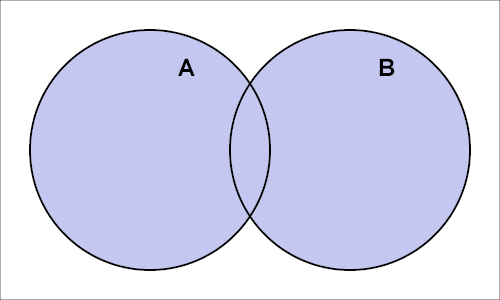
\includegraphics[width=10em]{image1.png}
        \caption{\(A\cup B\)}
    \end{subfigure}
    \quad
    \begin{subfigure}{10em}
        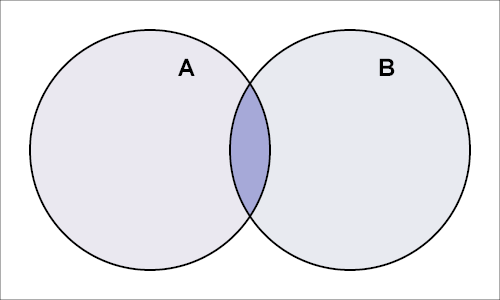
\includegraphics[width=10em]{image3.png}
        \caption{\(A\cap B\)}
    \end{subfigure}
    \quad
    \begin{subfigure}{10em}
        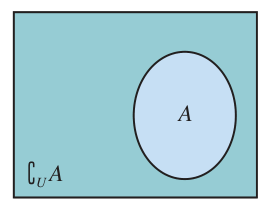
\includegraphics[width=10em]{image2.png}
        \caption{\(\complement_U A\)}
    \end{subfigure}
    \caption{并集、交集与补集}
\end{figure}

\subsection{补集}

\subsubsection{全集}

如果一个集合含有所研究问题中涉及的所有元素,那么就称这个集合为\textbf{全集}\index{全集 universal set},通常记作 \(U\).

\subsubsection{定义}

对于一个集合 \(A\),由全集 \(U\) 中不属于集合 \(A\) 的所有元素组成的集合称为集合 \(A\) 相对于全集 \(U\) 的\textbf{补集}\index{补集 complementary set},
简称为集合 \(A\) 的补集,记作 \(\complement_U A\).
\[
    \complement_U A = \{x| x\in U \text{且}x\not\in A\}
\]

\subsubsection{性质}

\begin{thmlevel1}[德摩根公式]\label{thm:demorgan}
    全集为 \(U\),集合 \(A,B\) 一定满足:
    \begin{gather*}
        \complement_U(A\cup B)=(\complement_U A)\cap(\complement_U B)\\
        \complement_U(A\cap B)=(\complement_U A)\cup(\complement_U B)
    \end{gather*}
\end{thmlevel1}

简记:\(\overline{A\cup B}=\overline{A}\cap \overline{B}\),\(\overline{A\cap B}=\overline{A}\cup \overline{B} \).证明可采用 Venn 图,从略.

\subsection{集合的元素个数}

我们把含有限个元素的集合叫作\textbf{有限集},用 \(\card(A)\) 来表示有限集合 \(A\) 中元素的个数.一个集合中元素的个数称为这个集合的基数.也有其他记法,例如:\(|A|\).

\begin{thmlevel1}[容斥原理]
    \(A,B,C\) 都是有限集,则:
    \begin{align*}
        |A\cup B|={}       & |A|+|B|-|A\cap B|               \\
        |A\cup B\cup C|={} & + |A|+|B|+|C|                   \\
                           & - |A\cap B|-|B\cap C|-|C\cap A| \\
                           & + |A\cap B\cap C|
    \end{align*}
\end{thmlevel1}

证明可采用 Venn 图,从略.

\section{充分条件与必要条件}

\subsection{充分条件与必要条件}

如果“若 \(p\),则 \(q\)”是真命题,那么称由 \(p\) 可以推出 \(q\),记作 \(p\Rightarrow q\),并且说,\(p\) 是 \(q\) 的\textbf{充分条件}\index{充分条件 sufficient condition},
\(q\) 是 \(p\) 的\textbf{必要条件}\index{必要条件 necessary condition}.

如果“若 \(p\),则 \(q\)”是假命题,那么由 \(p\) 不能推出 \(q\),记作 \(p\nRightarrow q\),此时,\(p\) 不是 \(q\) 的充分条件,\(q\) 不是 \(p\) 的必要条件.

举反例是判断一个命题是假命题的重要方法.

充分条件通常不唯一.判定定理给出了结论成立的一个充分条件.

必要条件通常不唯一.性质定理给出了结论成立的一个必要条件.

\subsection{充要条件}

如果“若 \(p\),则 \(q\)”和其逆命题“若 \(q\),则 \(p\)”均是真命题,即既有 \(p\Rightarrow q\),又有 \(q\Rightarrow p\),就记作 \(p \Leftrightarrow q\).
此时,\(p\) 既是 \(q\) 的充分条件,又是 \(q\) 的必要条件,我们说 \(p\) 是 \(q\) 的\textbf{充分必要条件},
简称为\textbf{充要条件}\index{充要条件 necessary and sufficient condition}.此时命题 \(p,q\) 等价.显然,如果 \(p\) 是 \(q\) 的的充要条件,那么 \(q\) 也是 \(p\) 的的充要条件.

\section{全称量词与存在量词}

\subsection{全称量词与存在量词}

短语“所有的”“任意一个”\footnote{常见的全称量词还有“一切”“每一个”“任给”等。}在逻辑中通常叫做\textbf{全称量词}\index{全称量词 universal quantifier},
并用符号“\(\forall\)”表示。含有全称量词的命题,叫作\textbf{全称量词命题},例如:\(\forall x \in M, p(x)\)。

短语“存在一个”“至少有一个”\footnote{常见的存在量词还有“有些”“有一个”“对某些”“有的”等。}在逻辑中通常叫做\textbf{存在量词}\index{存在量词 existential quantifier},
并用符号“\(\exists\)”表示。含有全称量词的命题,叫作\textbf{存在量词命题},例如:\(\exists x \in M,p(x)\)。

\subsection{全称量词命题和存在量词命题的否定}

否定一个命题 \(p(x)\),得到一个新命题,这一新命题称为原命题的否定,记作 \(\lnot p(x)\),即“\(p(x)\) 不成立”。

否定全称量词命题或存在量词命题时,只需要将全称量词改为存在量词,或把存在量词改为全称量词,然后对结论进行否定即可。

命题 \(\forall x \in M, p(x)\) 的否定是 \(\exists x \in M, \lnot p(x)\)。命题 \(\exists x \in M, p(x)\) 的否定是 \(\forall \in M, \lnot p(x)\)。

\chapter{复数} % 韦达定理,分圆方程,欧拉公式

\section{复数的概念}

\subsection{数系的扩充和复数的概念}

为了使方程 \(x^2=-1\) 有解,人们引入 \(\ii\),并规定 \(\ii\) 的平方等于 \(-1\),即
\[
    \ii^2=-1
\]

我们把形如 \(a+b \ii(a,b\in \mathbb{R})\) 的数叫作\textbf{复数}\index{复数 complex number},其中 \(\ii\) 叫作\textbf{虚数单位}\index{虚数单位 imaginary unit}。
全体复数构成的集合 \(\mathbb{C}=\{a+b \ii|a,b\in \mathbb{R}\}\) 叫作\textbf{复数集}\index{复数集 set of complex numbers}。不难
看出,\(\mathbb{R}\subsetneqq \mathbb{C}, \ii\in \mathbb{C}\)。

复数通常用字母 \(z\) 表示,即 \(z=a+b \ii(a,b\in \mathbb{R})\)。以后如不特殊声明,用 \(z=a+b \ii\) 等类似表达式表示复数时,都
有 \(a,b\in \mathbb{R}\),其中的 \(a\) 与 \(b\) 分别叫做复数 \(z\) 的\textbf{实部}\index{实部 real part}与\textbf{虚部}\index{虚部 imaginary part}。

本书中,用\(\Re(z)\)表示复数 \(z\) 的实部,用 \(\Im(z)\)表示复数\(z\)的虚部。注意:\(\Im(z)\in \mathbb{R} \)。

任取两个数 \(a+b \ii,c+d \ii\in \mathbb{C}\),规定:

\centerline{\(a+b \ii\) 和 \(c+d \ii\) 相等当且仅当 \(a=c\text{且} b=d\)}

对于复数 \(a+b \ii(a,b\in \mathbb{R})\),当且仅当 \(b=0\) 时,它是实数;当且仅当 \(a=b=0\) 时,它
是实数 \(0\);当 \(b \ne 0\) 时,它叫做\textbf{虚数}\index{虚数 imaginary number};当 \(a=0 \text{且} b \ne 0\) 时,它叫做\textbf{纯虚数}。

虚数之间、虚数与实数之间不能比较大小。

\subsection{复数的几何意义}

\subsubsection{几何意义1:复平面上的点}

实数与数轴上的点一一对应,因此实数可以用数轴上的点来表示。类似的,由于任何一个复数 \(z=a+b \ii\) 都可以由一个有序数对 \((a,b)\) 唯一确定,并且任何一个复数都可以唯一确定一个
有序实数对,所以复数 \(z=a+b \ii\) 与有序实数对 \((a,b)\) 一一对应。而有序实数对 \((a,b)\) 与平面直角坐标系中的点一一对应,所以复数集与平面直角坐标系中的点集之间
可以建立一一对应关系。

如图~\ref{fgr:fuuibnui1},点 \(Z\) 的横坐标是 \(a\),纵坐标是 \(b\),复数 \(z=a+b \ii\) 可用点 \(Z(a,b)\) 表示。这个建立了平面直角坐标系来表示复数
的平面叫作\textbf{复平面},\(x\) 轴叫作\textbf{实轴},\(y\) 轴叫作\textbf{虚轴},如图~\ref{fgr:fuuibnui3} 所示。实轴上的点都表示实数;除了原点外,虚轴上的点都表示纯虚数。

\begin{figure}
    \begin{subfigure}{3cm}
        \centering
        \begin{tikzpicture}
            \node[below left] (O) at (0,0) {$O$};
            \draw[->] (0,-0.5) -- (0,3) node[left] {$y$};
            \draw[->] (-0.5,0) -- (2,0) node[below] {$x$};
            \node[right] (Z) at (1,2) {$Z:a+b \ii$};
            \draw[dashed] (0,2) node[left] {$b$}-- (1,2);
            \draw[dashed] (1,0) node[below] {$a$} -- (1,2);
        \end{tikzpicture}
        \caption{复平面中的复数}\label{fgr:fuuibnui1}
    \end{subfigure}
    \hfill
    \begin{subfigure}{3cm}
        \centering
        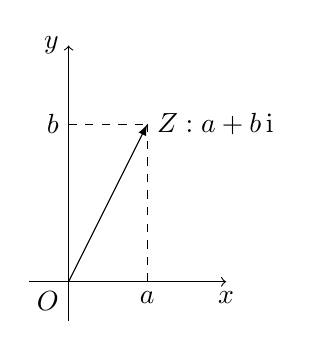
\begin{tikzpicture}
            \node[below left] (O) at (0,0) {$O$};
            \draw[->] (0,-0.5) -- (0,3) node[left] {$y$};
            \draw[->] (-0.5,0) -- (2,0) node[below] {$x$};
            \node[right] (Z) at (1,2) {$Z:a+b \ii$};
            \draw[dashed] (0,2) node[left] {$b$} -- (1,2);
            \draw[dashed] (1,0) node[below] {$a$} -- (1,2);
            \draw[-latex] (0,0) -- (1,2);
        \end{tikzpicture}
        \caption{复数与平面向量}\label{fgr:fuuibnui2}
    \end{subfigure}
    \hfill
    \begin{subfigure}{3cm}
        \centering
        \begin{tikzpicture}
            \node[below left] (O) at (0,0) {$O$};
            \draw[->] (0,-1.5) -- (0,1.5) node[left] {$y$};
            \draw[->] (-1.5,0) -- (1.5,0) node[below] {$x$};
            \draw[dashed,step=1] (-1,-1) grid (1,1);
            \node[below left] (i) at (0,1) {$\ii$};
            \node[below left] (-i) at (0,-1) {$\mathrm{-i}$};
            \node[below left] (1) at (1,0) {$1$};
            \node[below left] (-1) at (-1,0) {$-1$};
        \end{tikzpicture}
        \caption{复平面}\label{fgr:fuuibnui3}
    \end{subfigure}
    \caption{复数的几何表示}
\end{figure}

按照这种方法,每一个复数,有复平面内唯一的一个点和它对应;反过来,复平面内的每一个点,有唯一的一个复数和它对应。由此可知,复数集 \(\mathbb{C}\) 中的数与复平面内的点
按如下方式建立了一一对应关系:

\centerline{\tikz\draw[<->] (0,0) node[left] {复数 \(z=a+b \ii\)}-- node[above] {一一对应}(4em,0) node[right] {复平面内的点 \(Z(a,b)\)};}

这是复数的一种几何意义。

\subsubsection{几何意义2:平面向量}

如图~\ref{fgr:fuuibnui2},设复平面内的点 \(Z\) 表示复数 \(z=a+b \ii\),连 \(OZ\),显然向量 \(\vec{OZ}\) 由点 \(Z\) 唯一确定;反过来,点 \(Z\) 也可以由
向量 \(\vec{OZ}\) 唯一确定。由此可知,复数集 \(\mathbb{C}\) 中的数与以原点为起点的向量建立了如下一一对应关系(实数 \(0\) 与 \(\vec{0}\) 对应):

\centerline{\tikz\draw[<->] (0,0) node[left] {复数 \(z=a+b \ii\)}-- node[above] {一一对应}(4em,0) node[right] {平面向量 \(\vec{OZ}\)};}

这是复数的另一种几何意义。\footnote{人教A版第71页:这种几何表示也称阿尔冈图(Argand diagram)。}

\subsubsection{绝对值、共轭复数}

为方便起见,我们常把复数 \(z=a+b \ii\) 说成点 \(Z\) 或说成向量 \(\vec{OZ}\),并且规定,相等的向量表示同一个复数。

图~\ref{fgr:fuuibnui2} 中向量 \(\vec{OZ}\) 的模叫作\textbf{复数 \(z=a+b \ii\) 的模}\index{复数的模 modulus of a complex number}或\textbf{绝对值},记
作 \(|z|\) 或 \(|a+b \ii|\)。即
\[
    |z|=|a+b \ii|=\sqrt{a^2+b^2} \  (a,b \in \mathbb{R})
\]

如果 \(b=0\),则 \(|z|=|a|\),也就是 \(a\) 的绝对值。

一般地,当两个复数的实部相等,虚部互为相反数时,我们称这两个复数互为\textbf{共轭复数}\index{共轭复数 conjugate complex number}。虚部不等于 \(0\) 的两个共轭复数
也叫做共轭虚数。复数 \(z\) 的共轭复数用 \(\overline{z}\) 表示,即如果 \(z=a+b \ii\),那么 \(\overline{z}=a-b \ii\)。

一对共轭复数在复平面内对应的点关于实轴对称。

\section{复数的四则运算}

\subsection{复数的加减运算及其几何意义}

\subsubsection{复数的加法运算及其几何意义}

规定复数的加法法则如下:

设 \(z_1=a+b \ii,z_2=c+d \ii\) 是任意两个复数,其和
\[
    (a+b \ii)+(c+d \ii)=(a+c)+(b+d) \ii
\]

注意到,复数相加仍为复数。

容易验证,复数的加法满足交换律、结合律。共轭复数的和是实数。

如图~\ref{fgr:fuuujxfa},%
设 \(\vec{OZ_1},\vec{OZ_2}\) 分别与复数 \(a+b\ii,c+d\ii\) 对应,则 \(\vec{OZ_1}=(a,b),\vec{OZ_2}=(c,d)\)。我们有 \(\vec{OZ_1}+\vec{OZ_2}=(a+c,b+d)\),这说
明 \(\vec{OZ_1}+\vec{OZ_2}\) 就是复数 \((a+c)+(b+d) \ii\) 对应的向量。因此复数的加法可以按照向量的加法来进行,这就是复数加法的几何意义。

\subsubsection{复数的减法运算及其几何意义}

类比实数中相反数的定义,我们定义 \(-z\) 是复数 \(z\) 的\textbf{相反数}\footnote{人教A版中无此定义。},并规定:
\[
    -z=-(a+b\ii)=-a-b\ii
\]

我们把满足 \(z_1+(x+y)\ii=z_2(z_1,z_2 \in \mathbb{C})\) 的复数 \(x+y\ii\) 叫作复数 \(z_1\) 与 \(z_2\) 的差,记作 \(z_1-z_2\),并规定 \(z_1-z_2=z_1+(-z_2)\)。

不妨设 \(z_1=a+b\ii,z_2=c+d\ii\),则\[(c+d\ii)+(x+y\ii)=a+b\ii\]

根据复数相等的含义,
\begin{align*}
    c+x & = a,  & d+y & =b   \\
    x   & =a-c, & y   & =b-d
\end{align*}

因此
\begin{align*}
    z_1-z_2 & =(a+b\ii)-(c+d\ii) \\
            & =x+y\ii
            & =(a-c)+(b-d)\ii
\end{align*}

这就是复数的减法法则。

注意到,复数相减仍为复数。

\begin{figure}
    \centering
    \begin{subfigure}{10em}
        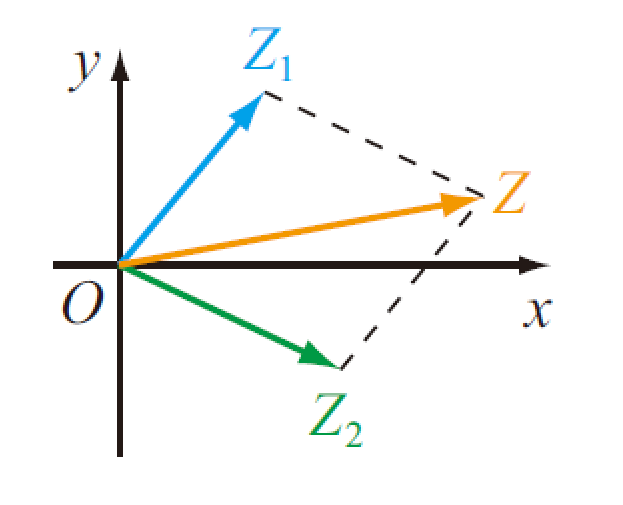
\includegraphics[width=10em]{image4.png}
        \caption{加法}\label{fgr:fuuujxfa}
    \end{subfigure}
    \qquad
    \begin{subfigure}{10em}
        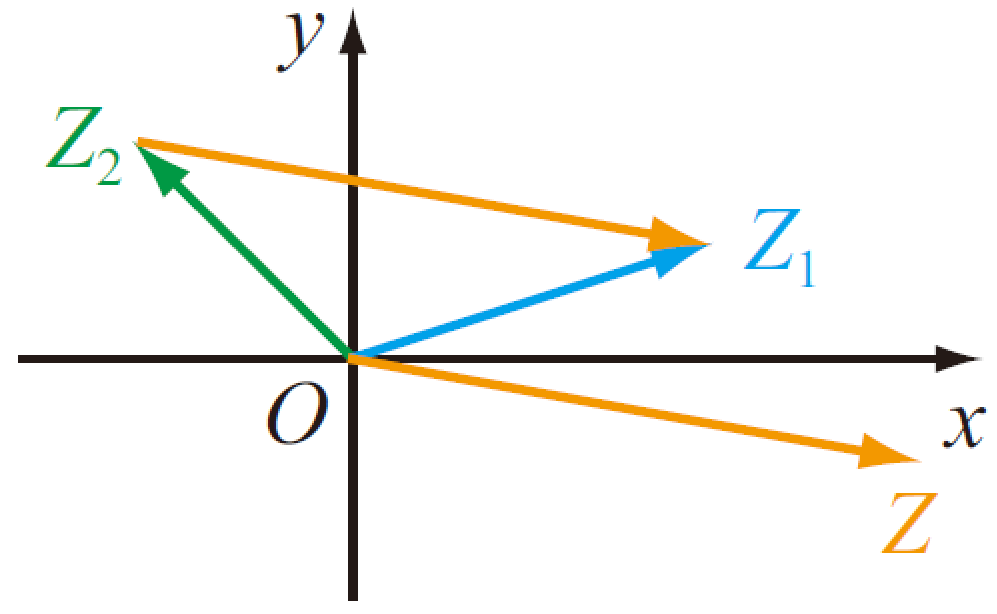
\includegraphics[width=10em]{image5.png}
        \caption{减法}\label{fgr:fuuujmfa}
    \end{subfigure}
    \caption{复数加减法的几何意义}
\end{figure}

由复数与向量之间的对应关系同样可以得出复数减法的几何意义:如果复数 \(z_1,z_2\) 所对应的向量分别为 \(\vec{OZ_1},\vec{OZ_2}\),设点 \(Z\) 满
足 \(\vec{OZ}=\vec{Z_2Z_1}\),则 \(z_1-z_2\) 所对应的向量就是 \(\vec{OZ}\),如图~\ref{fgr:fuuujmfa} 所示。由复数的几何意义可以得出复数的绝对值三角不等式,证明略。

\begin{thmlevel1}[复数的绝对值三角不等式]
    任意两个复数 \(z_1,z_2\) 一定满足
    \[
        \big||z_1|-|z_2|\big|\le |z_1-z_2| \le |z_1|+|z_2|
    \]
\end{thmlevel1}

\subsection{复数的乘除运算}

\subsubsection{复数的乘法}

一般地,设 \(z_1=a+b\ii,z_2=c+d\ii\),称 \(z_1z_2\)(或 \(z_1\times z_2\))为 \(z_1\) 与 \(z_2\) 的积,并规定
\begin{align*}
    z_1z_2 & = (a+b\ii)(c+d\ii)       \\
           & = ac+ad\ii+bc\ii+bd\ii^2 \\
           & =(ac-bd)+(ad+bc)\ii
\end{align*}

注意到,复数相乘仍为复数。

可以证明,复数的乘法运算满足交换律与结合律,且对加法满足分配律。

\subsubsection{复数的乘方}

\(n\) 个相同的复数 \(z\) 相乘时,仍称为 \(z\) 的 \(n\) 次\textbf{方}(或 \(n\) 次\textbf{幂}),并记作 \(z^n\),即
\[z^n=\underbrace{z\times z\times \cdots \times z}_{n\text{个}}\]

可以验证,当 \(m,n\) 均为正整数时,
\[z^mz^n=z^{m+n},(z^m)^n=z^{mn},(z_1z_2)^n=z_1^nz_2^n\]

\subsubsection{复数的除法}

如果复数 \(z_2\ne 0\),则满足 \(zz_2=z_1\) 的复数 \(z\) 称为 \(z_1\) 除以 \(z_2\) 的\textbf{商},\(z_1\) 为被除数,\(z_2\) 为除数。给
定复数 \(z\ne 0\),称 \(\dfrac{1}{z}\) 为 \(z\) 的\textbf{倒数}。

复数的除法法则:
\begin{align}
    (a+b\ii)\div (c+d\ii) & =\frac{a+b\ii}{c+d\ii}                                              \notag                \\
                          & =\frac{(a+b\ii)(c-d\ii)}{(c+d\ii)(c-d\ii)}                          \label{eq:ffmuuiuuhx} \\
                          & =\frac{ac+bd}{c^2+d^2}+\frac{bc-ad}{c^2+d^2}\ii \quad (c+d\ii\ne 0) \notag
\end{align}

其中,步骤(\ref{eq:ffmuuiuuhx}) 被称为“分母实数化”。显然,利用这种办法可以求出任意一个非零复数的倒数,以及任意两个复数的商(除数不能为 \(0\))。

注意到,复数相除仍为复数。

\subsection{复数四则运算的常用结论}

\begin{enumerate}
    \item \((1 \pm \ii)^2=\pm 2 \ii\),\(\dfrac{1+\ii}{1-\ii}=\ii\),\(\dfrac{1-\ii}{1+\ii}=-\ii\);
    \item \(-b+a\,\mathrm{i}=\ii(a+b\,\mathrm{i}) \ (a,b \in \mathbb{R} )\);
    \item \(\ii^{4n}=1,\ii^{4n+1}=\ii,\ii^{4n+2}=-1,\ii^{4n+3}=-\ii \quad (n \in \mathbb{N} ^*)\);
    \item \(|z^2|=|z|^2=|\overline{z}|^2=z \overline{z}\),\(\left|\overline{z}\right|=\overline{z}\),\(\overline{(\overline{z})}=z\);
    \item \(|z_1z_2|=|z_1||z_2|\),\(\left|\dfrac{z_1}{z_2}\right|=\dfrac{|z_1|}{|z_2|}(z_2 \ne 0)\),\(|z^n|=|z|^n\);
    \item \(\overline{z_1 \pm z_2}=\overline{z_1}\pm \overline{z_2}\),\(\overline{z_1z_2}=\overline{z_1}\, \overline{z_2}\),
          \(\overline{\left(\left|\dfrac{z_1}{z_2}\right|\right)}=\dfrac{|\overline{z_1}|}{|\overline{z_2}|}(z_2 \ne 0)\),
          \(\overline{z^n}=\overline{z}^n\ (n \in \mathbb{Z} )\)。
\end{enumerate}

从结论 5可以看出,复数的模运算可以与乘法、除法、乘方运算交换顺序;从结论6可以看出,复数的共轭运算可以与加减乘除以及乘方运算交换顺序。

\section{一元二次方程的复数解和代数基本定理}

\subsection{实系数一元二次方程在复数范围内的解集}

当 \(a,b,c\in \mathbb{R}\text{且}a\ne 0\) 时,关于 \(x\) 的方程 \(ax^2+bx+c=0\) 称为\textbf{实系数一元二次方程},这个方程
在复数范围内总是有解的,而且
\begin{enumerate}
    \item 当 \(\varDelta=b^2-4ac>0\) 时,方程有两个不相等的实数根;
    \item 当 \(\varDelta=b^2-4ac=0\) 时,方程有两个相等的实数根;
    \item 当 \(\varDelta=b^2-4ac<0\) 时,方程有两个互为共轭的虚数根。
\end{enumerate}

下面推导 \(\varDelta<0\) 时实系数一元二次方程 \(ax^2+bx+c=0\) 的求根公式。
\begin{align*}
    ax^2+bx+c                     & =0                                                             \\
    x^2+\frac{b}{a}x+\frac{c}{a}  & =0                                                             \\
    \left(x+\frac{b}{2a}\right)^2 & =\frac{b^2-4ac}{4a^2}                                          \\
    \left(x+\frac{b}{2a}\right)^2 & =-\frac{-(b^2-4ac)}{(2a)^2}                                    \\
    x+\frac{b}{2a}                & =\pm\frac{\sqrt{-(b^2-4ac)}}{2a}\ii                            \\
    x                             & =\frac{-b\pm\sqrt{4ac-b^2}\ii}{2a} \quad (\varDelta=b^2-4ac<0)
\end{align*}

注意到,此时两根的虚部的绝对值相等,两根互为共轭。

\begin{thmlevel1}[二次韦达定理]\label{thm:erciwwdadkli}
    在复数域内,关于 \(x\) 的方程 \(ax^2+bx+c=0(a\ne 0)\) 的两根 \(x_1,x_2\) 满足:
    \[
        \begin{cases}
            x_1+x_2=-\dfrac{b}{a} \\
            x_1x_2=\dfrac{c}{a}
        \end{cases}
    \]
\end{thmlevel1}

证明可采用求根公式代入,从略。

\subsection{代数基本定理}

\begin{thmlevel1}[代数基本定理]
    任何一元\(n(n\in \mathbb{N^*})\)次复系数多项式方程\(f(x)=0\)至少有一个复数根。
\end{thmlevel1}

证明方法很多,但是每一种证明方法都涉及高等数学,从略。

由代数基本定理可以证明,任何一元\(n(n\in \mathbb{N^*})\)次复系数多项式\(f(x)\)在复数集中可以分解为\(n\)个一次因式的乘积。进而,一元\(n(n\in \mathbb{N^*})\)次多项式
方程有\(n\)个复数根(重根按照重数计)。证明如下:

\begin{proof}
    采用数学归纳法。

    (归纳奠基)对于一次多项式
    \[
        f(x) = a_1x + a_0 \quad (a_1 \neq 0)
    \]
    方程 \( f(x) = 0 \) 的解是:
    \begin{gather}
        x = -\frac{a_0}{a_1} \label{eq:yiciwwda}
    \end{gather}
    有且仅有一个根,结论成立。

    (归纳假设)假设对于所有次数 \( \leq n-1 \) 的复系数多项式,结论成立。即:任何 \( k \) 次复系数多项式(\( k \leq n-1 \))在复数域上恰有 \( k \) 个根(重根按重数计)。

    (归纳步骤)设 \( f(x) \) 是一个 \( n \) 次复系数多项式:
    \[
        f(x) = a_nx^n + a_{n-1}x^{n-1} + \cdots + a_0 \quad (a_n \neq 0)
    \]

    由代数基本定理,\( f(x) = 0 \) 至少有一个复根,记为 \( \alpha \),于是\(f(x)\) 可分解为
    \[
        f(x) = (x - \alpha) \cdot q(x)
    \]
    其中 \( q(x) \) 是一个 \( n-1 \) 次的复系数多项式。

    根据归纳假设,\( q(x) = 0 \) 有 \( n-1 \) 个复根(重根按重数计),记为 \( \beta_1, \beta_2, \dots, \beta_{n-1} \)。

    综上,根据数学归纳法,\(\forall n\in \mathbb{N^*}\),\( f(x) = 0 \) 的全体根为:
    \[
        \alpha, \beta_1, \beta_2, \dots, \beta_{n-1}
    \]
    共 \( n \) 个根(如果 \( \alpha \) 与某些 \( \beta_i \) 相同,则计算重数)。
\end{proof}

这个证明过程的核心是使用因式分解(因式定理)来降低次数,同时,代数基本定理保证了归纳基础。

\subsection{一元多项式方程根与系数的关系}

次数为\(1\)的情况即式(\ref{eq:yiciwwda})。次数为\(2\)的情况即第 \pageref{thm:erciwwdadkli} 页的二次韦达定理。

设实系数一元三次方程
\begin{gather}
    a_3x^3+a_2x^2+a_1x+a_0=0 \quad (a_3\ne 0) \label{eq:sjciwwdafhig}
\end{gather}
在复数集 \(\mathbb{C}\) 内的根为 \(x_1,x_2,x_3\),可以得到方程(\ref{eq:sjciwwdafhig}) 的变形
\[
    a_3(x-x_1)(x-x_2)(x-x_3)=0
\]
展开得
\begin{gather}
    a_3x^3-a_3(x_1+x_2+x_3)x^2+a_3(x_1x_2+x_1x_3+x_2x_3)x-a_3x_1x_2x_3=0 \label{eq:sjciwwdavjkd}
\end{gather}
比较式(\ref{eq:sjciwwdafhig})(\ref{eq:sjciwwdavjkd})可以得到
\[
    \begin{cases}
        x_1+x_2+x_3=-\dfrac{a_2}{a_3}         \\
        x_1x_2+x_1x_3+x_2x_3=\dfrac{a_1}{a_3} \\
        x_1x_2x_3=-\dfrac{a_0}{a_3}
    \end{cases}
\]

更高次一元多项式方程根与系数的关系不在本节讨论范围内。

\section{复数的三角表示}

\subsection{复数的三角表示式}

一般地,如果非零复数 \(z=a+b\,\mathrm{i}\) 在复平面内对应点 \(Z(a,b)\),且 \(r\) 为向量 \(OZ\) 的模, \(\theta\) 是以 \(x\) 轴非负半轴为始边、射线 \(OZ\) 为终边
的一个角,则
\[
    r=|z|=\sqrt{a^2+b^2}
\]
根据正余弦的定义
\begin{align*}
    \cos \theta=\frac{a}{r},\quad & \sin \theta=\frac{b}{r} \\
    a=r \cos \theta,        \quad & b=r \sin \theta
\end{align*}
如图~\ref{fgr:fuuusjjn} 所示,从而
\[z=a+b\,\mathrm{i}=(r \cos \theta)+(r \sin \theta)\,\mathrm{i}\]

其中,\(r\) 是复数 \(z\)的模,\(\theta\)称为 \(z\) 的\textbf{辐角}\index{辐角 argument}。
\((r \cos \theta)+(r \sin \theta)\,\mathrm{i}\)称为非零复数 \(z=a+b\,\mathrm{i}\) 的\textbf{三角表示式},简称\textbf{三角形式}。对应地,\(a+b\,\mathrm{i}\)称为复数的\textbf{代数表示式}),简称\textbf{代数形式}。

显然,任何一个非零复数 \(z\) 的辐角都有无穷多个,而且任意两个辐角之间都相差 \(2\pi\) 的整数倍。特别地,在 \([0,2 \pi )\)内的辐角
称为 \(z\) 的\textbf{辐角主值},记作 \(\arg z\)。

每一个非零复数有唯一的模与辐角主值,二者唯一确定该复数。两个非零复数相等当且仅当它们的模与辐角主值分别相等(但是辐角可以相差\(2 \pi \)的整数倍)。

\begin{figure}
    \centering
    \begin{minipage}{13em}
        \centering
        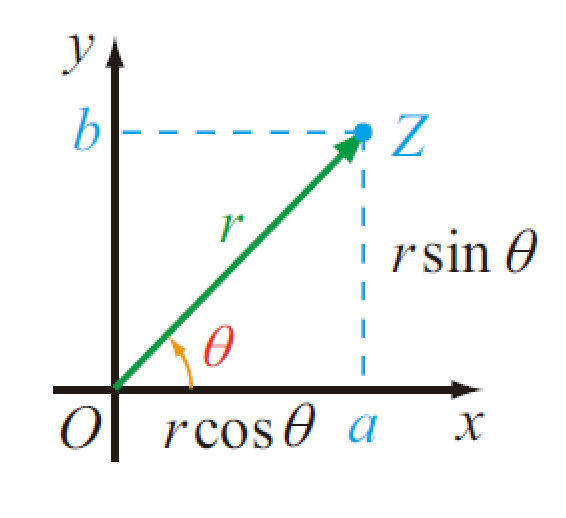
\includegraphics[width=10em]{image7.png}
        \caption{复数的三角表示}\label{fgr:fuuusjjn}
    \end{minipage}
    \qquad
    \begin{minipage}{13em}
        \centering
        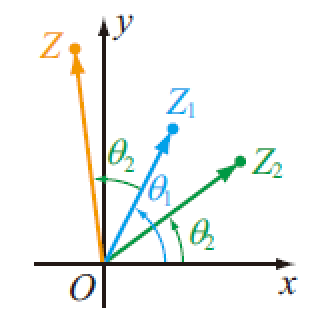
\includegraphics[width=10em]{image8.png}
        \caption{复数乘法的几何意义}\label{fgr:fuuusjjnigfa}
    \end{minipage}
\end{figure}

\subsection{复数乘除运算的三角表示及其几何意义}

\subsubsection{乘法}

设复数 \(z_1=r_1(\cos \theta_1 + \,\mathrm{i} \sin \theta _1),z_2=r_2(\cos \theta_2 + \,\mathrm{i} \sin \theta _2)\),则
\begin{align*}
    z_1z_2 & =r_1(\cos \theta_1 + \,\mathrm{i} \sin \theta _1)\cdot r_2(\cos \theta_2 + \,\mathrm{i} \sin \theta _2)                                   \\
           & =r_1r_2(\cos \theta_1 + \,\mathrm{i} \sin \theta _1)(\cos \theta_2 + \,\mathrm{i} \sin \theta _2)                                         \\
           & =r_1r_2[(\cos \theta _1 \cos \theta _2-\sin \theta _1 \sin \theta _2)+\ii(\sin \theta _1 \cos \theta _2 + \cos \theta _1 \sin \theta _2)] \\
           & =r_1r_2[\cos (\theta _1+\theta _2)+\ii \sin (\theta _1+\theta _2)]
\end{align*}
即
\[
    r_1(\cos \theta_1 + \,\mathrm{i} \sin \theta _1)\cdot r_2(\cos \theta_2 + \,\mathrm{i} \sin \theta _2)
    =r_1r_2[\cos (\theta _1+\theta _2)+\ii \sin (\theta _1+\theta _2)]
\]

这就是说,两个复数相乘,积的模等于各复数的模之积,积的辐角等于各复数的辐角之和。

两个复数\(z_1,z_2\)相乘时,可以像图~\ref{fgr:fuuusjjnigfa} 一样,通过把向量逆时针旋转\(\theta _2\)角、按\(r_2\)伸长得到乘积所对应的向量。这就是复数乘法的几何意义。

不难看出,上述两个复数三角形式的乘法及其几何意义,可以推广到有限个复数的三角形式相乘。事实上,

\marginpar{
    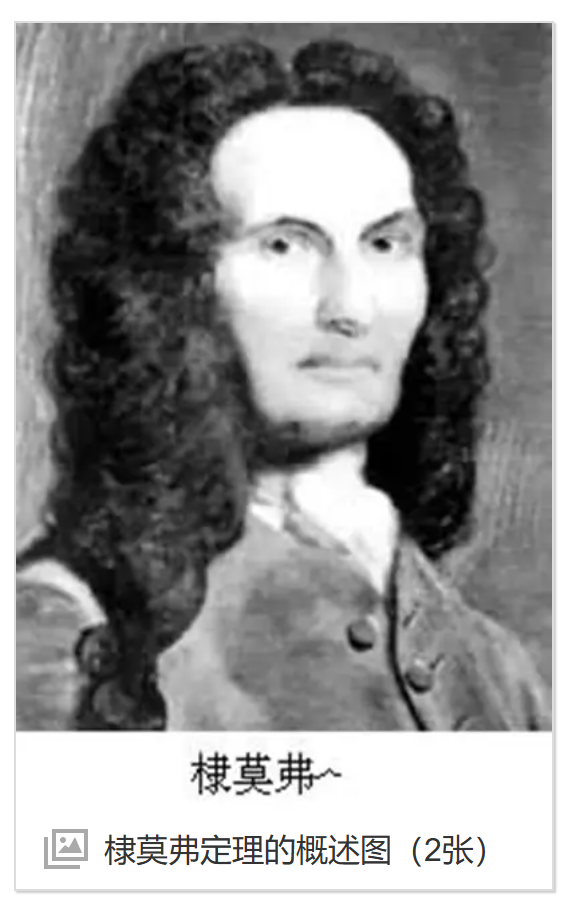
\includegraphics[width=0.9\marginparwidth]{image9.png}\\
    \footnotesize 图源:百度百科
}

\begin{thmlevel1}[棣莫弗公式]
    \(\forall x\in \mathbb{R}, n\in \mathbb{Z}\),\[( \cos (x) + i \sin (x) )^n = \cos (nx) + i \sin (nx)\]
\end{thmlevel1}

证明可以先通过数学归纳法证明正整数的情况,再推广到负整数。注意,不可以使用欧拉公式进行证明,因为欧拉公式的证明中用到了棣莫弗公式,会造成循环论证。

\begin{proof}
    先证\(P ( n ) = ( \cos \theta + \ii \sin \theta )^n =\cos (n \theta) + \ii \sin (n \theta) , n \in\mathbb{N}\)。采用数学归纳法。

    (归纳奠基)当\(n=0\)时,显然成立。当\(n=1\)时:\\
    左式\( = ( \cos \theta + \ii \sin \theta )^1 =  \cos \theta + \ii \sin \theta  = \cos (1 \cdot \theta) + \ii \sin (1 \cdot \theta) =  \)右式

    因此,\(P(1)\)成立。

    (归纳假设)当\(n>1\)时:假设\(P(k)\)成立,即\((\cos\theta + \ii\sin\theta)^k = \cos (k\theta) + \ii\sin(k\theta)\)。

    (归纳步骤)当\(n=k+1\)时:
    \begin{align*}
          & (\cos\theta + \ii\sin\theta)^{k+1}                                                                                                              \\
        = & (\cos\theta + \ii\sin\theta)^{k} \cdot (\cos\theta + \ii\sin\theta)                                                                             \\
        = & (\cos k\theta + \ii\sin k\theta)  \cdot (\cos\theta + \ii\sin\theta)                                                                            \\
        = & (\cos k\theta  \cdot \cos\theta + \ii\sin k\theta  \cdot \ii\sin\theta) + (\cos k\theta  \cdot \ii\sin\theta+\ii\sin k\theta  \cdot \cos\theta) \\
        = & (\cos k\theta  \cdot \cos\theta - \sin k\theta  \cdot \sin\theta) + \ii(\cos k\theta  \cdot \sin\theta + \sin k \theta  \cdot \cos\theta)       \\
        = & \cos (k\theta+\theta) + \ii\sin (k\theta+\theta)                                                                                                \\
        = & \cos [(k+1)\theta] + \ii\sin [(k+1)\theta]
    \end{align*}

    因此,\(P(k+1)\)也成立。

    综上,根据数学归纳法,\(\forall n \in \mathbb{N}\),\(P(n)\)成立。

    另外,由恒等式\( (\cos (n \theta)+\ii \sin (n \theta)) \cdot (\cos (-n \theta)+\ii \sin (-n \theta)) =1 \)可知,公式对于负整数情况也成立。
\end{proof}

\subsubsection{除法}

复数的除法运算是乘法运算的逆运算。

设 \(z_1=r_1(\cos \theta_1 + \,\mathrm{i} \sin \theta _1),z_2=r_2
(\cos \theta_2 + \,\mathrm{i} \sin \theta _2)\quad (z_2 \ne 0)\),因为
\[
    r_2(\cos \theta_2 + \,\mathrm{i} \sin \theta _2)\cdot\frac{r_1}{r_2}[\cos (\theta _1-\theta _2)+
        \ii \sin (\theta _1-\theta _2)]=r_1(\cos \theta_1 + \,\mathrm{i} \sin \theta _1)
\]
所以根据复数除法的定义,有
\[
    \boxed{
        \frac{r_1(\cos \theta_1 + \,\mathrm{i} \sin \theta _1)}{r_2(\cos \theta_2 + \,\mathrm{i} \sin \theta _2)}=\frac{r_1}{r_2}[\cos (\theta _1-\theta _2)+
            \ii \sin (\theta _1-\theta _2)]
    }
\]

这就是说,两个复数相除,商的模等于被除数的模除以除数的模所得的商,商的辐角等于被除数的辐角减去除数的辐角所得的差。

\subsection{单位根}

\(n\) 次单位根是 \(n\) 次幂为 \(1\) 的复数。它们位于复平面的单位圆上,构成正多边形的顶点。

\subsubsection{定义}

方程 \(z^n=1\quad (n=1,2,3,\dots)\) 的复数根 \(z\) 为 \(n\) 次单位根,有 \(n\) 个:
\[\cos \frac{2 \pi k}{n}+\,\mathrm{i} \sin \frac{2 \pi k}{n}\quad (k=0,1,2,\dots,n-1)\]

\subsubsection{复平面中的体现}

当 \(n \ge 3\) 时,在复平面中单位根对应的点依次相连得到正 \(n\) 边形,其中一定有一个顶点落在 \((1,0)\) 处。

当 \(n=4\)时,\(4\)个单位根分别是 \(1,\ii,-1,-\ii\),如图~\ref{fgr:fuuibnui3}(第 \pageref{fgr:fuuibnui3} 页)所示。

\subsubsection{3次单位根}

下面研究 \(n=3\)时的情况。

设 \(z= \rho (\cos \varphi +\ii \sin \varphi )(\rho >0)\) 是 \(1\) 的 \(3\)次方根,则 \(z^3=1=\cos 0+\ii \sin 0\),从而
\[
    [\rho (\cos \varphi +\ii \sin \varphi )]^3=\rho ^3(\cos (3 \varphi )+\ii \sin (3 \varphi ))=\cos 0+\ii \sin 0
\]

由复数相等的定义,
\[
    \begin{cases}
        \rho ^3=1 \\
        3 \varphi =0+2k \pi \ (k \in \mathbb{Z} )
    \end{cases}
\]
即
\[
    \begin{cases}
        \rho ^3=1 \\
        \varphi=\dfrac{2k \pi }{3} \ (k \in \mathbb{Z} )
    \end{cases}
\]

因此 \(1\) 的 \(3\) 次方根是 \(\omega_k=\cos \dfrac{2k \pi }{3}+\ii \sin \dfrac{2k \pi }{3}\ (k \in \mathbb{Z} )\)。根据三角函数的周
期性,得\(\omega_0=1,\omega_1=-\dfrac{1}{2}+\dfrac{\sqrt{3}}{2}\ii,\omega_2=-\dfrac{1}{2}-\dfrac{\sqrt{3}}{2}\ii\)。

\begin{wrapfigure}{r}{8em}
    \centering
    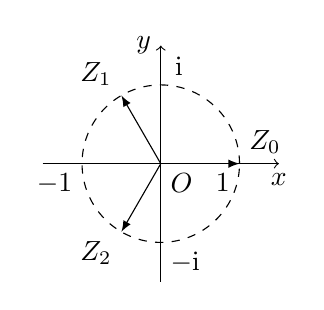
\begin{tikzpicture}
        \node[below right] at (0,0) {$O$};
        \draw[->] (0,-1.5) -- (0,1.5) node[left] {$y$};
        \draw[->] (-1.5,0) -- (1.5,0) node[below] {$x$};
        \draw[dashed] (0,0) circle (1);
        \node[above right] (i) at (0,1) {$\ii$};
        \node[below right] (-i) at (0,-1) {$\mathrm{-i}$};
        \node[below left] (1) at (1,0) {$1$};
        \node[below left] (-1) at (-1,0) {$-1$};
        \draw[-latex] (0,0) -- (1,0) node[above right]{\(Z_0\)};
        \draw[-latex] (0,0) -- (-0.5,0.866025403784) node[above left]{\(Z_1\)};
        \draw[-latex] (0,0) -- (-0.5,-0.866025403784) node[below left]{\(Z_2\)};
    \end{tikzpicture}
    \caption{\(3\)次单位根}\label{fgr:3cidjwwgf}
\end{wrapfigure}

如图~\ref{fgr:3cidjwwgf} 所示,在复平面内,设 \(\omega_0,\omega_1,\omega_2\) 对应的点分别为 \(Z_0,Z_1,Z_2\),显然 \(Z_0,Z_1,Z_2\) 都在单位圆上。
因为 \(\omega_0,\omega_1,\omega_2\) 的辐角依次相差 \(\dfrac{2 \pi }{3}\),所以\(Z_0,Z_1,Z_2\)三等分圆周。\(Z_0\)恰为单位圆与实轴正半轴交点。

不难看出,\(3\)次单位根有如下性质:

\begin{enumerate}
    \item \((\omega_k)^3=1,|\omega_k|=1\),其中 \(k=0,1,2\);
    \item \(\omega_1=\overline{\omega_2}\);
    \item \(1+\omega_k+\omega_k^2=0 \ (k=1,2)\)。
\end{enumerate}

事实上,人们常用如下方法表示 \(3\) 次单位根:\(1,\omega,\overline{\omega}\),其中\(\omega=-\dfrac{1}{2}+\dfrac{\sqrt{3}}{2}\ii\)

\subsubsection{单位根的和式}

当 \(n \ge 2\)时,\(n\)次单位根之和为 \(0\) 。

证明方法有很多,一种几何证法是转化为向量,利用单位圆的内接正多边形的重心在原点的性质,即 \(\sum \vec{OZ}_i=\vec{0}\) 进行处理。具体过程从略。

\chapter{函数与不等式}

\section{函数的概念及其表示}

\subsection{函数的概念}

\marginpar{\footnotesize 17世纪后期,德国数学家莱布尼茨第一次将“function”作为专门的数学术语;19世纪,李善兰首次将其翻译为“函数”(“凡此变数中函彼变数者,则此为彼之函数”)。}
一般地,设 \(A,B\) 为非空实数集,如果 \(\forall x \in A\),按照某种对应关系 \(f\),在 \(B\) 中都有唯一确定的元素 \(y\) 与之对应,那么就称 \(f:A\rightarrow B\)
为集合 \(A\) 到集合 \(B\) 的一个\textbf{函数}\index{函数 function},记作\[y=f(x),x\in A\]
其中,\(x\) 叫作自变量,\(x\)的取值范围 \(A\)叫作函数的\textbf{定义域}\index{定义域 domain},\(B\) 则叫作到达域。
如果自变量取值 \(a\),则由对应关系 \(f\) 确定的值 \(y\) 叫作函数 \(f\) 在 \(a\) 处的函数值,记作 \(y=f(x)\) 或 \(y |_{x=a}\);
函数值的集合\({f(x)|x\in A}\)叫作函数的\textbf{值域}\index{值域 range}。

这里给出函数的集合论表示法下的正式定义:

二元关系 \(f\) 若满足\marginpar{\footnotesize 这里说的是,\(x\)对应 \(y\)和\(y^\prime\),则二者相等。你细品!\(\wedge \)是逻辑学中的“且”,\(\vee \)则是“或”。}
\[
    (\forall x)(\forall y)(\forall y^{\prime})
    \{\,
    [\,(\langle x,\,y \rangle \in f)
            \wedge
            (\langle x,\,y^{\prime}\rangle \in f)\,]
    \Rightarrow (y=y^{\prime})
    \,\}
\]
则称\(f\)为一函数。为了与逻辑叙述的括弧作区分,这里用\(\langle x,y \rangle\)表示有序对。

注意以下几点:
\begin{enumerate}
    \item 当使用 \(f(a)\) 记号时,必有\(f\)为一函数且 \(a\in A\),其中 \(A\) 是函数 \(f\)的定义域;\footnote{事实上,如果这两个条件并不都满足,则\(f(a)=\varnothing\)。}
    \item 函数\(f\) 的值域是记号\(f:A\rightarrow B\)中的\(B\)的子集。若值域 \(R_f=B\),则映射 \(f:A\rightarrow B\)为满射;
    \item 函数也可以用 \(g,h\) 等其他字母表示;
    \item 定义域和对应关系分别相同的两个函数为同一个函数(字母不必相同);
    \item 在表示函数时,如果不会产生歧义,函数的定义域通常省略不写,此时就约定:函数的定义域就是使得这个函数有意义的所有实数组成的集合。
\end{enumerate}

函数就像是一个机器,同样的输入下,一定会给出同样的结果,如图~\ref{fgr:functionmachine} 所示。因此,对等式两边作同样的函数操作,等式依然成立。

\begin{figure}
    \centering
    \begin{minipage}{10em}
        \centering
        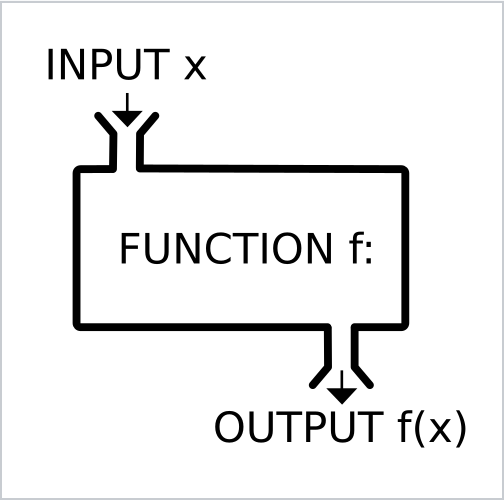
\includegraphics[width=10em]{image10.png}
        \caption{函数就像机器}\label{fgr:functionmachine}
    \end{minipage}
    \hfill
    \begin{minipage}{10em}
        \centering
        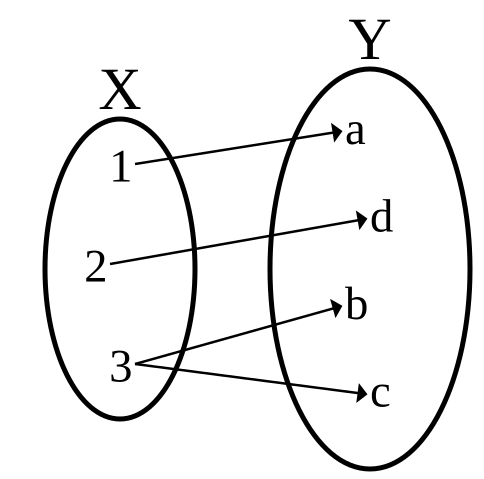
\includegraphics[width=10em]{image11.png}
        \caption{多值函数不是函数}
    \end{minipage}
    \hfill
    \begin{minipage}{10em}
        \centering
        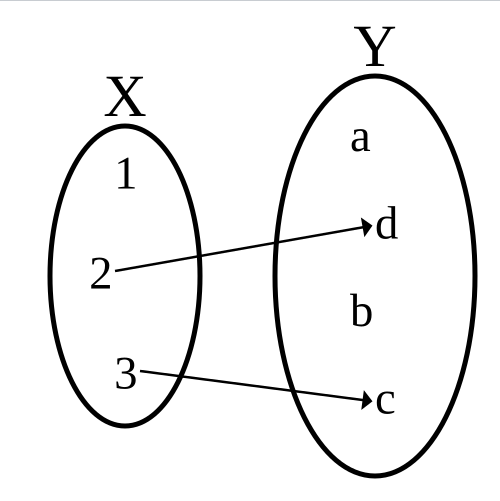
\includegraphics[width=10em]{image12.png}
        \caption{偏函数不是函数}
    \end{minipage}
\end{figure}

\subsection{区间}

如表~\ref{tbl:qujmuuvzbnui} 所示,区间指的是满足某一不等式的取值 \(x\) 的\textit{集合},其中的\(a,b\)\textit{须}满足 \(a<b\)。其中的第1、2、3、4类区间又分别称为闭区间、开
区间、左闭右开区间、左开右闭区间,左闭右开区间与左开右闭区间统称为半开半闭区间,简称半开区间。其中的实数 \(a,b\) 叫作相应区间的端点,但 \(+\infty \) 和 \(-\infty \)不是。

实数集 \(\mathbb{R} \) 可以用区间表示为 \((-\infty ,+\infty )\),“\(\infty \)”读作“无穷大”,“\(-\infty \)”读作“负无穷大”,“\(+\infty \)”读作“正无穷大”。

\begin{table}
    \centering
    \begin{tabular}{ccc}
        \toprule
        区间记法                                                             & 数轴表示                                                                          & 对应不等式 \\
        \midrule
        \([a,b]\)                                                            & \parbox{4cm}{\tikz{ \draw[->] (0,0) -- (4,0); \draw[solid] (1,0)
                node[below]{$a$}--(1,0.3) -- (3,0.3) -- (3,0) node[below]{$b$}; \fill (1,0)
        circle(2pt);\fill(3,0) circle (2pt); }}                              & \(a \le x \le b\)                                                                              \\ \((a,b)\)                                                 & \parbox{4cm}{\tikz{ \draw[->] (0,0) -- (4,0); \draw[solid] (1,0) node[below]{$a$}
                   -- (1,0.3) -- (3,0.3) -- (3,0) node[below]{$b$}; \filldraw[fill=white] (1,0)
        circle (2pt);\filldraw[fill=white] (3,0) circle (2pt); }}            & \(a < x < b\)                                                                                  \\
        \([a,b)\)                                                            & \parbox{4cm}{\tikz{ \draw[->] (0,0) -- (4,0); \draw[solid] (1,0) node[below]{$a$}
                -- (1,0.3) -- (3,0.3) -- (3,0) node[below]{$b$}; \fill (1,0) circle
        (2pt);\filldraw[fill=white] (3,0) circle (2pt); }}                   & \(a \le x < b\)                                                                                \\
        \((a,b]\)                                                            & \parbox{4cm}{\tikz{ \draw[->] (0,0) -- (4,0); \draw[solid] (1,0) node[below]{$a$}
                -- (1,0.3) -- (3,0.3) -- (3,0) node[below]{$b$}; \filldraw[fill=white] (1,0)
        circle (2pt);\fill (3,0) circle (2pt); }}                            & \(a < x \le b\)                                                                                \\ \([a,+\infty )\)
                                                                             & \parbox{4cm}{\tikz{ \draw[->] (0,0) -- (4,0); \draw[solid] (1,0) node[below]{$a$}
        -- (1,0.3) -- (4,0.3); \fill (1,0) circle (2pt);}}                   & \(x \ge a\)                                                                                    \\
        \((a,+\infty)\)                                                      & \parbox{4cm}{\tikz{ \draw[->] (0,0) -- (4,0); \draw[solid] (1,0) node[below]{$a$}
        -- (1,0.3) -- (4,0.3); \filldraw[fill=white] (1,0) circle (2pt); }}  & \(x>a\)
        \\ \((- \infty ,b]\)                                    & \parbox{4cm}{\tikz{ \draw[->] (0,0) -- (4,0); \draw[solid] (0,0.3) -- (3,0.3) --
        (3,0) node[below]{$b$}; \fill (3,0) circle (2pt); }}                 & \(x \le b\)                                                                                    \\
        \((-\infty ,b)\)                                                     & \parbox{4cm}{\tikz{ \draw[->] (0,0) -- (4,0); \draw[solid] (0,0.3) -- (3,0.3) --
        (3,0) node[below]{$b$}; \filldraw[fill=white] (3,0) circle (2pt); }} & \(x<b\)
        \\ \bottomrule
    \end{tabular}
    \caption{区间与数轴表示}\label{tbl:qujmuuvzbnui}
\end{table}

\subsection{函数的表示}

函数的三种常用的表示法为:解析法、列表法和图象法。

\begin{description}
    \item[解析法] 用解析式表示两个变量之间的对应关系,如 \(f(x)=x^2\)。
    \item[列表法] 列出表格来表示两个变量之间的对应关系。
    \item[图象法] 用图象表示两个变量之间的对应关系。
\end{description}

如果函数 \(f:A \rightarrow B\) 满足\(\forall x \in A,f(x)=T_x\),其中 \(T_x\) 是一个含 \(x\) 的项,那么 \(f\) 可以用箭号表示为:
\[f:A\rightarrow B;\ x\mapsto T_x\]

这样的 \(f\) 可以用间隔号简记为 \(T_{(\cdot)}\),例如 \(f:\mathbb{R} \rightarrow \mathbb{R} ;\ x\mapsto x^2\) 简记为 \((\cdot)^2\)。这种记法的缺点是无法指出定义域。
\marginpar{
    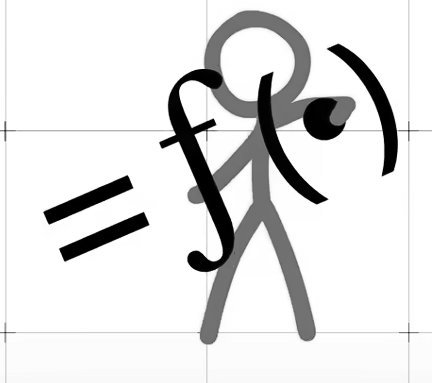
\includegraphics[width=0.9\marginparwidth]{image13.png}\\
    \footnotesize 再临:6
}

一元函数如果定义域和值域都是 \(\mathbb{R} \)的子集,那么可以使用图象法来表示。判断一个图形是否是函数图象的方法是垂线检验,即图形
与任何一条平行于 \(y\) 轴的直线不能有超过一个交点。

有的函数,定义域是离散的点,这样的函数图象是一系列离散的点,研究时可以用虚线连接;有的函数,图象无法用形象描绘,例如狄利克雷函数:%
\marginpar{\footnotesize 狄利克雷函数是一种0-1指示函数,这类函数用于指示哪些元素属于定义域的某
    一子集\(S\)。除了 \(\mathbf{1}_S(x)\) 以外,也用 \(\chi _S(x)\) 或 \(I_S(x)\)表示。}
\[
    \mathbf{1}_\mathbb{Q}(x)=\begin{cases}
        1, & x\in \mathbb{Q}       \\
        0, & x \not \in \mathbb{Q}
    \end{cases}
    \quad (x \in \mathbb{R})
\]

有的函数,其自变量在不同的取值区间内,函数有不同的对应关系,称这样的函数为\textbf{分段函数},将会在~\ref{1db9720b-d3ee-41cf-b2a7-ec5f8e8cd900} 节进行探讨。

\section{函数的基本性质}

\subsection{函数的单调性与最值}

\subsubsection{单调性的定义}

一般地,设函数 \(y=f(x)\) 的定义域为 \(D\),且区间 \(I \subseteq D\):
\begin{enumerate}
    \item 如果 \(\forall x_1,x_2 \in I,x_1<x_2\),都有\(f(x_1)<f(x_2)\),则称该函数在区间 \(I\)上\textbf{单调递增}或该函数在区间 \(I\)上是增函数;
    \item 如果 \(\forall x_1,x_2 \in I,x_1<x_2\),都有\(f(x_1)>f(x_2)\),则称该函数在区间 \(I\)上\textbf{单调递减}或该函数在区间 \(I\)上是减函数。
\end{enumerate}

在两种情况下,都称该函数在区间 \(I\) 上具有单调性,区间 \(I\) 叫作该函数的单调区间。单调区间包括所有这样的具有单调性的区间。

特别地,在定义域上单调递增、单调递减的函数分别称为\textbf{增函数}、\textbf{减函数}。

结合不等式的性质容易得到,若 \(f(x),g(x)\) 都是增函数,则函数 \(h(x)=f(x)+g(x)\) 也为增函数。其他情况同理,读者自证不难。

作为例子,下面证明函数 \(f(x)=\sqrt{x}\) 是增函数。

\begin{proof}
    函数的定义域是 \([0,+\infty )\)。

    \(\forall x_1,x_2 \in [0,+\infty )\),且\(x_1<x_2\),有
    \begin{align*}
        f(x_1)-f(x_2) & =\sqrt{x_1}-\sqrt{x_2}                                                         \\
                      & =\dfrac{(\sqrt{x_1}-\sqrt{x_2})(\sqrt{x_1}+\sqrt{x_2})}{\sqrt{x_1}+\sqrt{x_2}} \\
                      & =\dfrac{x_1-x_2}{\sqrt{x_1}+\sqrt{x_2}}
    \end{align*}
    因为 \(x_1-x_2<0,\sqrt{x_1}+\sqrt{x_2}>0\),所以 \(f(x_1)<f(x_2)\),即函数\(f(x)=\sqrt{x}\) 是增函数。
\end{proof}

证明的关键步骤是第二个等号,巧妙运用平方差公式,把无法比较大小的\(1\over 2\)次式转化为 \(1\)次式,并且保证了分母为正。不妨把这叫作“分子有理化”。

\subsubsection{最值的定义}

一般地,设函数 \(y=f(x)\) 的定义域为 \(D\),如果存在实数 \(M\) 满足:
\begin{enumerate}
    \item \(\forall x \in D\),都有 \(f(x)\le M\);
    \item \(\exists x_0 \in D\),使得 \(f(x_0)=M\)。
\end{enumerate}

那么,称该函数的\textbf{最大值}\index{最大值 maximum value}是\(M\),\(x_0\)是该函数的一个\textbf{最大值点}。

一般地,设函数 \(y=f(x)\) 的定义域为 \(D\),如果存在实数 \(M\) 满足:
\begin{enumerate}
    \item \(\forall x \in D\),都有 \(f(x)\ge M\);
    \item \(\exists x_0 \in D\),使得 \(f(x_0)=M\)。
\end{enumerate}

那么,称该函数的\textbf{最小值}\index{最小值 minimum value}是\(M\),\(x_0\)是该函数的一个\textbf{最小值点}。

若函数在某一闭区间内单调,则区间的端点为函数的最值点。

\subsubsection{函数的平均变化率}

一般地,设函数 \(y=f(x)\) 的定义域为 \(D\),区间 \(I \subseteq D\),\(\forall x_1,x_2 \in I,x_1 \ne x_2\),
记 \(y_1=f(x_1),y_2=f(x_2),\dfrac{\Delta y}{\Delta x}=\dfrac{y_2-y_1}{x_2-x_1}\),则:
\begin{enumerate}
    \item 该函数在区间 \(I\) 上是增函数的充要条件是 \(\dfrac{\Delta y}{\Delta x}>0\) 在区间 \(I\)上恒成立;
    \item 该函数在区间 \(I\) 上是减函数的充要条件是 \(\dfrac{\Delta y}{\Delta x}<0\) 在区间 \(I\)上恒成立。
\end{enumerate}

一般地,当 \(x_1 \ne x_2\) 时,称
\[
    \dfrac{\Delta y}{\Delta x}=\dfrac{f(x_2)-f(x_1)}{x_2-x_1}
\]
为函数 \(y=f(x)\) 在区间 \([x_1,x_2]\)(\(x_1<x_2\)时)或 \([x_2,x_1]\)(\(x_1>x_2\)时)上的平均变化率。\footnote{人教A版中无此定义。}

注意:在高中数学的定义中,单调函数不允许出现不增不减的情况,即 \(\dfrac{\Delta y}{\Delta x}\) 不能为 \(0\)。

上述结论与单调性的定义本质相同,利用不等式的性质即可相互转化。二者均可用以证明函数的单调性。

\subsection{奇偶性与图象对称}

\subsubsection{奇偶性的定义}

一般地,设函数 \(y=f(x)\) 的定义域为 \(D\),如果 \(\forall x \in D\),都有 \(-x \in D\),且 \(f(-x)=f(x)\),那么该函数为\textbf{偶函数}\index{偶函数 even function}。

一般地,设函数 \(y=f(x)\) 的定义域为 \(D\),如果 \(\forall x \in D\),都有 \(-x \in D\),且 \(f(-x)=-f(x)\),那么该函数为\textbf{奇函数}\index{奇函数 odd function}。

奇偶性是函数在其定义域上的整体性质,所以判断函数的奇偶性前应先明确其定义域。

既是奇函数又是偶函数的函数是 \(y=0\)。注意到,若 \(x=0\) 在某个奇函数 \(f(x)\) 的定义域内,则 \(f(0)=-f(0)=0\)。

\subsubsection{奇偶函数图象特点}

偶函数的图象关于 \(y\) 轴呈轴对称,奇函数的图象关于原点呈中心对称。

\subsubsection{复合函数的奇偶性}

约定:“若 \(f(x),g(x)\) 都是奇函数,则函数 \(h(x)=f(x)+g(x)\) 也为奇函数”简记为“奇+奇=奇”。有如下结论成立:

奇 \(\pm\) 奇 = 奇,偶 \(\pm\) 偶=偶;偶 \(\times\) 偶=偶,奇 \(\times\) 奇=偶,奇 \(\times\) 偶=奇。除法与乘法同理。

使用定义容易证明。

复合函数 \(g(f(x))\) 的奇偶性判断方法:\marginpar{\footnotesize 有偶即偶,全奇才奇!}
\begin{enumerate}
    \item 若 \(f(x)\) 为奇函数,则 \(g(f(x))\) 的奇偶性同 \(g(x)\);
    \item 若 \(f(x)\) 为偶函数,则 \(g(f(x))\) 为偶函数,不论 \(g(x)\) 是否有奇偶性。
\end{enumerate}

证明思路很显然,若 \(f(x)\) 为偶函数,则自变量取相反数\(f(x)\)不变,再由函数值的唯一确定
性,\(g(f(x))\)也不变;若 \(f(x)\) 为奇函数,则自变量取相反数,则\(f(x)\)变为相反数,相当于 \(g(x)\) 的变量 \(x\)取相反数。

\subsubsection{常见的奇偶函数模型}

以下 \(y\) 关于 \(x\) 的函数为奇函数:
\begin{gather*}
    y=Ax^{2n+1},\ y=a^x-a^{-x},\ y=\log_a\left( \sqrt{x^2+1}\pm x \right),\ y=A\sin \omega x,\\
    y=A \tan \omega x ,\ y=\dfrac{a^x-a^{-x}}{a^x+a^{-x}},\ y=\log_a\dfrac{1-x}{1+x} \quad (a>0,\, a\ne 1,\, n \in \mathbb{Z} )
\end{gather*}

以下 \(y\) 关于 \(x\) 的函数为偶函数:
\begin{align*}
    y=Ax^{2n},\ y=a^x+a^{-x},\ y=\log_a\left( 1+a^{2kx} \right)-kx,\ y=A\cos \omega x, \\
    y=f(|x|),\ y=\mathrm{const.},\ y=A|x| \quad (a>0,\, a\ne 1,\, n \in \mathbb{Z} ,\, k\ne 0)
\end{align*}

下证\(f(x)=\log_a\left( \sqrt{x^2+1}\pm x \right)\ (a>0,a\ne 1)\) 为奇函数。

\begin{proof}
    \begin{align*}
        f(x) & =\log_a\left( \dfrac{\left( \sqrt{x^2+1}\pm x \right)\left( \sqrt{x^2+1}\mp x \right)}{\sqrt{x^2+1}\mp x} \right) \\
             & =\log_a\left( \dfrac{1}{\sqrt{x^2+1}\mp x} \right)                                                                \\
             & =-\log_a \left( \sqrt{x^2+1}\mp x \right)                                                                         \\
             & =-f(-x)
    \end{align*}
\end{proof}

下证\(y=\log_a\left( 1+a^{2kx} \right)-kx\ (a>0,a\ne 1,k\ne 0)\) 为偶函数。

\begin{proof}
    \begin{align*}
        f(-x) & =\log_a\left( 1+a^{-2kx} \right)+kx                 \\
              & =\log_a\left( \dfrac{a^{2kx}+1}{a^{2kx}} \right)+kx \\
              & =\log_a \left( 1+a^{2kx} \right)-2kx+kx             \\
              & =\log_a \left( 1+a^{2kx} \right)-kx                 \\
              & =f(x)
    \end{align*}
\end{proof}

其余函数奇偶性的证明十分显然,从略。

有的函数,可以恒等变形为上述函数的线性表达式。例如,函数 \(f(x)=\dfrac{3^x}{3^x + 1}\) 可以转化
为\(f(x)=\dfrac{1}{2}\cdot\dfrac{3^x-1}{3^x+1}+\dfrac{1}{2}\),下面给出推导。

设常数 \(m\),
\begin{align*}
    f(x) & =\dfrac{3^x}{3^x + 1} +m-m                                  \\
         & =\dfrac{3^x+m\cdot 3^x+m}{3^x + 1}-m                        \\
         & = \dfrac{(m+1)\left( 3^x+\dfrac{m}{m+1} \right)}{3^x + 1}-m
\end{align*}
令 \(\dfrac{m}{m+k}=-1\),得 \(m=-\dfrac{1}{2}\),代入得 \(f(x)=\dfrac{1}{2}\cdot\dfrac{3^x-1}{3^x+1}+\dfrac{1}{2}\)。

在此推导过程中,核心是抓住目标 \(f(x)=k\cdot \dfrac{3^x- 1}{3^x + 1}+b\),并且运用“加一减一”的技巧和待定系数法。

\subsubsection{函数图象的对称}

若函数 \(f(x)\) 的图象关于直线 \(x=a\) 对称,则 \(f(a-x)=f(a+x) \Leftrightarrow f(x)=f(2a-x)\);
若函数 \(f(x)\) 的图象关于点 \((a,b)\) 对称,则 \(b-f(a-x)=f(a+x)-b \Leftrightarrow f(x)+f(2a-x)=2b\)。

其中,第一个推论结合图形易得,等价推论通过 \(x'=a-x\) 的换元也容易证明。

注意到,当函数\(f(x)\)图象呈中心对称或轴对称时,在等式的同侧,\(f(k_1x+m)\pm f(k_2x+n)\) 中 \(k_1,k_2\) 满足 \(k_1+k_2=0\)。事实上这也是分析问题的重要依据。%
\marginpar{\footnotesize 大胆猜想,小心求证!}

\subsubsection{双对称求周期问题}

当已知条件中包含两个对称条件时,通常函数具有周期性。

(情形一)若函数 \(f(x)\) 的图象关于两条直线 \(x=a,x=b(a\ne b)\)对称,则函数 \(f(x)\) 为周期函数,且 \(2|a-b|\) 为函数 \(f(x)\) 的一个周期。证明如下:

\begin{proof}
    由已知,\(f(x)=f(2a-x),\ f(y)=f(2b-y)\),设 \(y=2a-x\),得 \(f(x)=f(2a-x)=f(y)=f(2b-y)=f(2b-(2a-x))=f(2(b-a)+x)\)。结论显然。
\end{proof}

(情形二)若函数 \(f(x)\) 的图象关于两个点 \((a,0),(b,0)(a \ne b)\) 对称,则函数 \(f(x)\) 为周期函数,且 \(2|a-b|\) 为函数 \(f(x)\) 的一个周期。证明同理,从略。

(情形三)若函数 \(f(x)\) 的图象关于直线 \(x=a\) 和点 \((b,0)\) 对称,则函数 \(f(x)\) 为周期函数,且 \(4|a-b|\) 为函数的一个周期或 \(f(x)=0\)。证明如下:

\begin{proof}
    由已知,\(f(x)=f(2a-x),\ f(y)+f(2b-y)=0\),设 \(y=2a-x\),得 \(f(x)=(2a-x)=f(y)=-f(2b-y)=-f(2(b-a)+x)\),当 \(a=b\)时,\(f(x)=0\);否则,再
    设 \(z=2(b-a)+x\),得 \(f(x)=-f(z)=-(-f(2(b-a)+z))=f(2(b-a)+2(b-a)+x)=f(4(b-a)+x)\)。结论显然。
\end{proof}

注意到,证明过程中出现了 \(f(x)=-f(x+k)\ (k\ne 0)\) 的形式,这是周期函数的典型特征(\(x\)前系数相同),由于\(f(\dots)\)前系数不同,再次换元代入即
可得到最小正周期为 \(2|k|\)。

\section{幂函数、分段函数与绝对值函数}

\subsection{幂函数}

一般地,形如 \(y=x^\alpha\) 的函数叫作\textbf{幂函数}\index{幂函数 power function}。其中 \(x\) 是自变量,\(\alpha\)是常数。

对于幂函数,我们只研究 \(\alpha=1,2,3,\frac{1}{2},-1\)时的图象与性质。

在同一坐标系下画出 \(\alpha=1,2,3,\dfrac{1}{2},-1\) 时 \(y=x^\alpha\) 的图象,如图~\ref{fgr:mihjuutuxl} 所示。

\begin{figure}
    \centering
    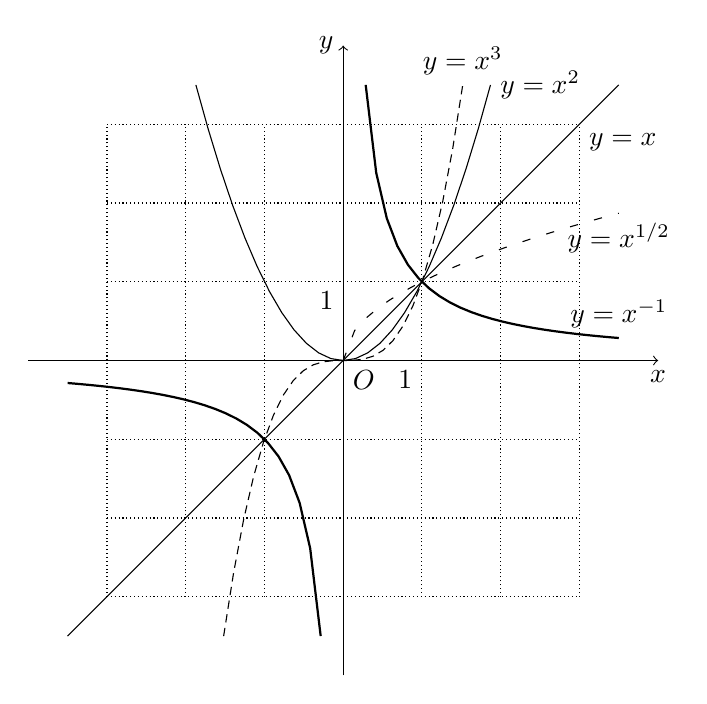
\begin{tikzpicture}
        \node[below right] at (0,0) {$O$};
        \node[below left] at (1,0) {$1$};
        \node[below left] at (0,1) {$1$};
        \draw[->] (-4,0) -- (4,0) node[below] {$x$};
        \draw[->] (0,-4) -- (0,4) node[left] {$y$};
        \draw[densely dotted,step=1] (-3,-3) grid (3,3);
        \draw[solid,domain=-3.5:3.5] plot(\x,{\x});
        \node[below right] at (3,3){$y=x$};
        \draw[thin,domain=-1.870828:1.870828] plot(\x,{\x*\x});
        \node[right] at (1.870828,3.5){$y=x^2$};
        \draw[densely dashed,domain=-1.518294:1.518294] plot(\x,{\x*\x*\x});
        \node[above] at (1.518294,3.5){$y=x^3$};
        \draw[loosely dashed,domain=0:3.5] plot(\x,{sqrt(\x)});
        \node[below] at (3.5,1.870828){$y=x^{1/2}$};
        \draw[thick,domain=-3.5:-0.285714] plot(\x,{1/\x});
        \draw[thick,domain=0.285714:3.5] plot(\x,{1/\x});
        \node[above] at (3.5,0.285714){$y=x^{-1}$};
    \end{tikzpicture}
    \caption{幂函数图象}\label{fgr:mihjuutuxl}
\end{figure}

事实上:

\begin{enumerate}
    \item 幂函数\(y=x^\alpha\)的图象在第一象限一定存在,且必定经过点 \((1,1)\),一定不经过第四象限;
    \item 当 \(\alpha >0\)时,幂函数图象过原点,且在 \([0,+\infty )\) 上单调递增;当 \(\alpha<0\) 时,幂函数图象不过原点,且在 \((0,+\infty )\)上单调递减;
    \item 在直线 \(x=1\) 的右边,\(\alpha\) 越大,函数值增长越快。
\end{enumerate}

通过探究 \(\alpha=1,2,3,\dfrac{1}{2},-1\) 时 \(y=x^\alpha\) 的图象,还可以得到幂函数的很多其他性质,在此不一一列举。

\subsection{分段函数}\label{1db9720b-d3ee-41cf-b2a7-ec5f8e8cd900}

分段函数是通常记为 \(f(x)=\begin{cases}
    f_1(x), & x \in D_1 \\
    f_2(x), & x \in D_2 \\
    \vdots              \\
    f_n(x), & x \in D_n
\end{cases}\) 的函数,自变量在不同的取值区间有“不同的”映射关系。沿用函数就像机器的比喻,分段函数就像是多个机器,对于不同的输入,会给入不同的机器产生返回。事实
上,选择机器+输入机器的过程,可以视为一个机器,因为分段函数也是函数,也就具有函数的一切特性,所以可以看作是一个“割裂的”映射关系。

在解决分段函数有关问题时,需要注意函数的定义域,不同取值区间不应有重叠。在实际问题中,不同的取值区间的并集往往是一个连续的区间,因此需要特别考虑区间断开处的
函数值情况,是否有跳跃等。

分段函数的的定义域为每一段自变量取值范围的并集。分段函数的值域为每一段函数值范围的并集,最大值是每一段最大函数值的最大值,最小值是每一段函最小数值的最小值。

\subsection{绝对值函数及其衍生}

\subsubsection{绝对值函数}

绝对值函数的分段定义如下:
\[
    |x|=\begin{cases}
        x,  & x \ge 0 \\
        -x, & x <0
    \end{cases}
\]

\begin{figure}
    \begin{minipage}{5cm}
        \centering
        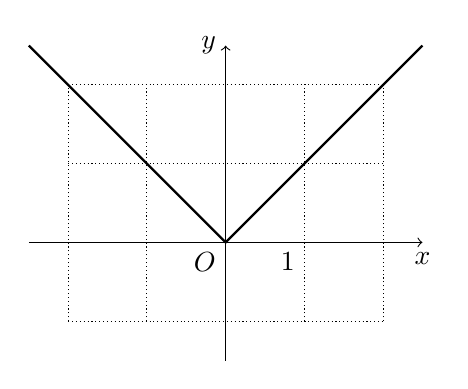
\begin{tikzpicture}
            \draw[->] (-2.5,0) -- (2.5,0) node[below] {$x$};
            \draw[->] (0,-1.5) -- (0,2.5) node[left] {$y$};
            \node[below left] at (0,0) {$O$};
            \node[below left] at (1,0) {$1$};
            \draw[densely dotted,step=1] (-2,-1) grid (2,2);
            \draw[thick,domain=-2.5:2.5] plot(\x,{abs(\x)});
        \end{tikzpicture}
        \caption{函数 \(y=|x|\) 图象}\label{7803bf0a-ff7b-4b83-ace9-8002b9468114}
    \end{minipage}
    \hfill
    \begin{minipage}{6cm}
        \centering
        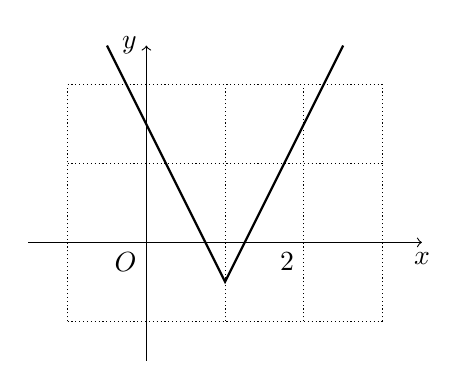
\begin{tikzpicture}
            \draw[->] (-1.5,0) -- (3.5,0) node[below] {$x$};
            \draw[->] (0,-1.5) -- (0,2.5) node[left] {$y$};
            \node[below left] at (0,0) {$O$};
            \node[below left] at (2,0) {$2$};
            \draw[densely dotted,step=1] (-1,-1) grid (3,2);
            \draw[thick,domain=-0.5:2.5] plot(\x,{2*abs(\x-1)-0.5});
        \end{tikzpicture}
        \caption{函数 \(y=2|x-1|-0.5\) 图象}\label{59b8dea0-9e48-4165-b6f8-e53600401b19}
    \end{minipage}
\end{figure}

函数 \(y=|x|\) 的图象如图~\ref{7803bf0a-ff7b-4b83-ace9-8002b9468114} 所示。

这是最基本的绝对值函数模型,可以看成是从原点引出两条关于过原点的竖直线(即 \(y\) 轴)对称的射线。

\subsubsection{一般绝对值函数}

对绝对值函数图象进行变换,得到更一般的形式:\(y=k|tx-a|+b\ (t \ne 0)\)。其中 \(k\) 控制右侧
这条射线的斜率,射线的端点则移动到了点 \((a,b)\) 处,\(|t|\)控制 \(x\) 坐标轴伸(\(<1\))缩(\(>1\))的程度。本小节中把这样的绝对
值函数称为一般绝对值函数。图~\ref{59b8dea0-9e48-4165-b6f8-e53600401b19} 是 \(k=2,a=1,b=-0.5,t=1\) 时的图象。

当我们把这样两个一般绝对值相加时,会得到一个新的绝对值函数,即 \(f(x)=k_1|t_1x-a_1|+k_2|t_2x-a_2|+b\ (t_1t_2\ne 0)\)。

解决此类问题的主要思想是分类讨论去掉绝对值,转化为一般分段函数,数形结合进行研究。下面研究 \(\dfrac{a_1}{t_1}\ne \dfrac{a_2}{t_2}\)的情况。根据各个参数的取值
不同,可分为如下四种类型(命名仅为便于记忆,仅在本小节适用)。

\subsubsection{平底锅模型}

形如 \(f(x)=|x-a|+|x-b|\) 的函数,由于其图象酷似平底锅,故称之为平底锅模型。在绝对值前乘上相同常数同理,不再赘述。

我们需要通过分类讨论将其转化为一般分段函数,各个击破。不妨设 \(a<b\)。可能分段的点为 \(x=a,x=b\) 两处,二者
把定义域 \(\mathbb{R} \)分为 \((-\infty ,a),[a,b],(b,+\infty )\) 三段。

分别考虑每一段上的情况,此时绝对值内的正负完全确定,可以去掉绝对值,得
\[
    f(x)=
    \begin{cases}
        -2x+a+b, & x<a          \\
        b-a,     & a \le x\le b \\
        2x-a-b,  & x>b
    \end{cases}
\]

注意到,当\(x\in [a,b]\) 时,函数值为定值 \(b-a\);两侧射线的斜率绝对值为 \(2\)。图~\ref{fgr:pkdigomoxk} 是 \(a=-1,b=1\) 时的函数图象。

关于函数值为定值的原因,有一个巧妙的几何解释。

如图~\ref{fgr:pkdigodepkdi},考虑数轴上 \(a,b,x\) 对应的点,则 \(f(x)\) 描述的是\(x\)对应点到 \(a,b\)对应点的距离之和。当\(x\)位于二者之间,也就
是 \(x\in [a,b]\)时,二者距离之和恰好等于 \(a,b\) 对应点之间的距离。

\begin{figure}
    \centering
    \begin{minipage}{5cm}
        \centering
        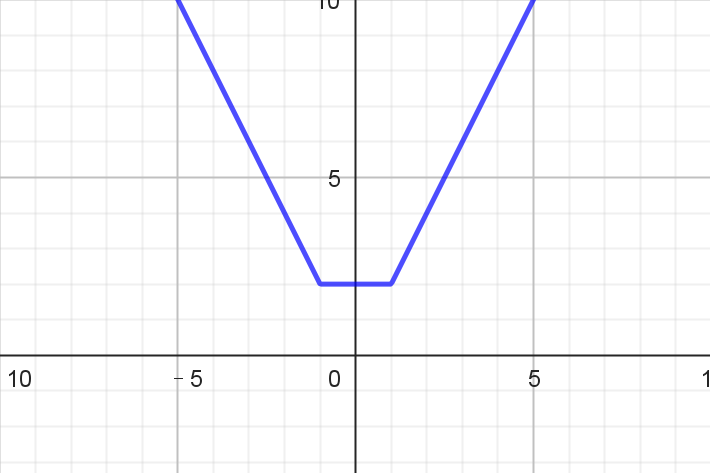
\includegraphics[width=5cm]{image14.png}
        \caption{平底锅模型}\label{fgr:pkdigomoxk}
    \end{minipage}
    \hfill
    \begin{minipage}{7cm}
        \centering
        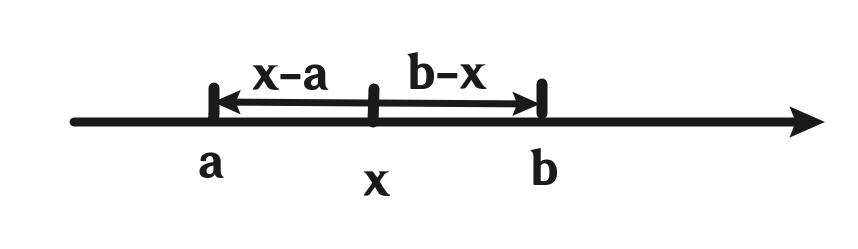
\includegraphics[width=7cm]{image15.png}
        \caption{平底锅的平底}\label{fgr:pkdigodepkdi}
    \end{minipage}
\end{figure}

如果再加上\(n\)个形如 \(|x-m|\) 的项,则图象将会为平底锅(\(n\) 为偶数)或尖底锅(\(n\)为奇数),如图~\ref{268282bf-8b1e-44db-853c-353758d4d5a7} 所示。

\begin{figure}
    \centering
    \begin{subfigure}{0.45\textwidth}
        \centering
        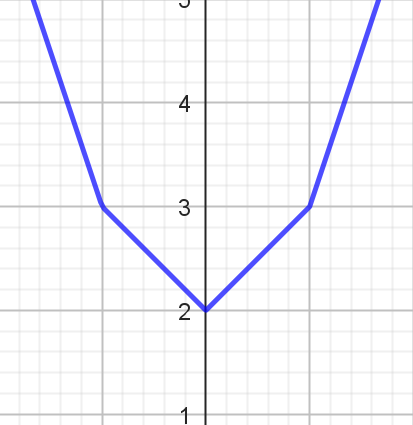
\includegraphics[width=\textwidth]{image17.png}
        \caption{\(y=|x+1|+|x|+|x-1|\)}
    \end{subfigure}
    \hfill
    \begin{subfigure}{0.45\textwidth}
        \centering
        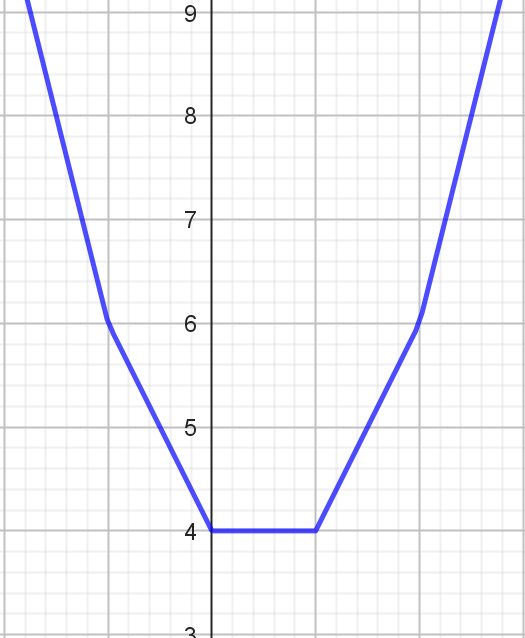
\includegraphics[width=\textwidth]{image16.png}
        \caption{\(y=|x+1|+|x|+|x-1|+|x-2|\)}
    \end{subfigure}
    \caption{尖底锅与平底锅函数图象}\label{268282bf-8b1e-44db-853c-353758d4d5a7}
\end{figure}

\subsubsection{Z字形模型}

形如 \(f(x)=|x-a|-|x-b|\) 的函数为该类型,其中 \(a\ne b\)。在绝对值前乘上相同常数同理,不再赘述。

分类讨论展开即可,同前。展开后又可分为以下两种情形:

(情形一)如图~\ref{db33b811-305c-4344-8c3f-90fdf39d069b},当\(a>b\)时,
\[f(x)=
    \begin{cases}
        |a-b|,   & x \le b \\
        -2x+a+b, & b<x<a   \\
        -|a-b|,  & x \ge a
    \end{cases}
\]

(情形二)如图~\ref{a8b3197b-0756-47ac-b002-05f20349e2e4},当\(a<b\)时,
\[f(x)=
    \begin{cases}
        |a-b|,  & x\le a \\
        2x-a-b, & a<x<b  \\
        -|a-b|, & x\ge b
    \end{cases}
\]

\begin{figure}
    \centering
    \begin{subfigure}{0.45\textwidth}
        \centering
        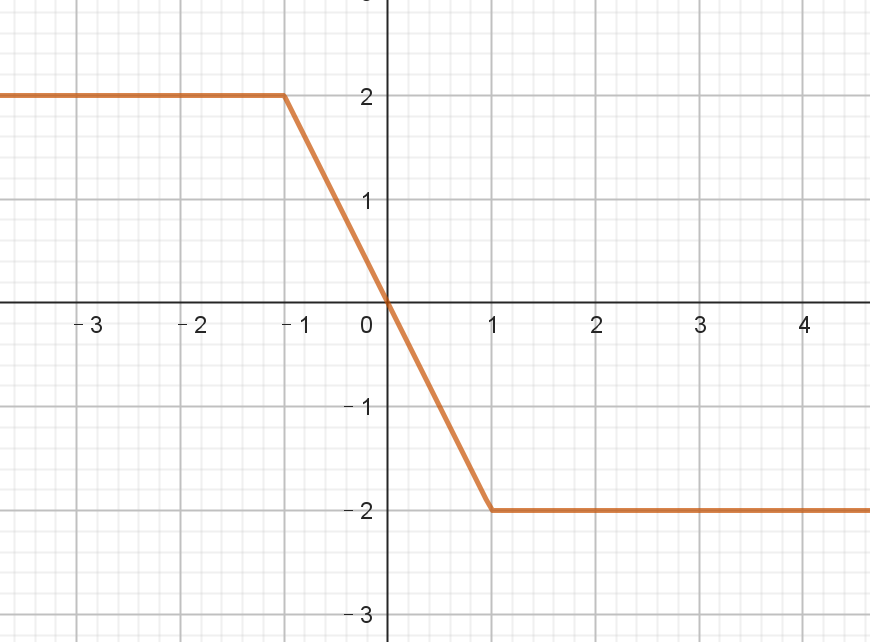
\includegraphics[width=\textwidth]{image18.png}
        \caption{$a=1,b=-1$}\label{db33b811-305c-4344-8c3f-90fdf39d069b}
    \end{subfigure}
    \hfill
    \begin{subfigure}{0.45\textwidth}
        \centering
        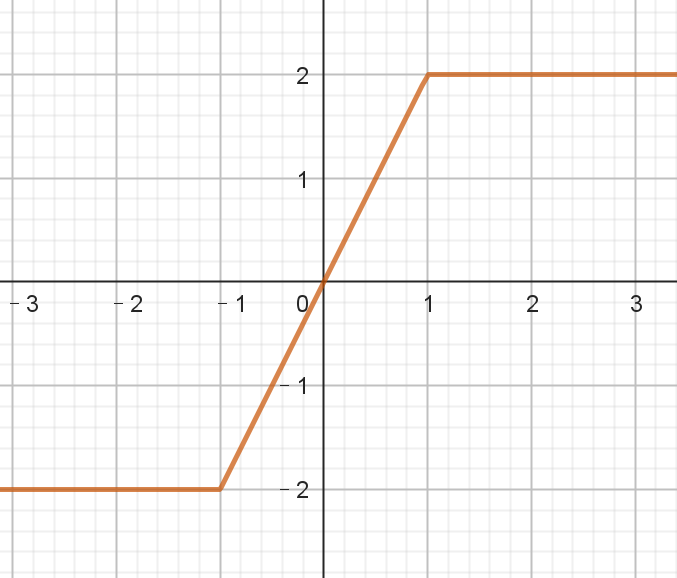
\includegraphics[width=\textwidth]{image19.png}
        \caption{$a=-1,b=1$}\label{a8b3197b-0756-47ac-b002-05f20349e2e4}
    \end{subfigure}
    \caption{Z字形模型}
\end{figure}

注意到,\marginpar{\footnotesize 大减小,大到小;小减大,没文化!}当 \(a-b>0\) 时,中间段函数值逐渐减小;当 \(a-b<0\) 时,中间段函数值逐渐增大。

\subsubsection{歪底锅模型}

形如 \(f(x)=m|x-a|+n|x-b|\ (a<b)\) 的属于该类型。下面研究 \(m,n>0\) 的情况。分类讨论同前。展开得
\[
    f(x)=
    \begin{cases}
        (-m-n)x+am+bn, & x<a   \\
        -an+bn,        & x=a   \\
        (m-n)x+am-bn,  & a<x<b \\
        -am+bm,        & x=b   \\
        (m+n)x-am-bn,  & x>b
    \end{cases}
\]

函数图象如图~\ref{fgr:wddigomoxk} 所示。
\begin{figure}
    \centering
    \begin{subfigure}{0.45\textwidth}
        \centering
        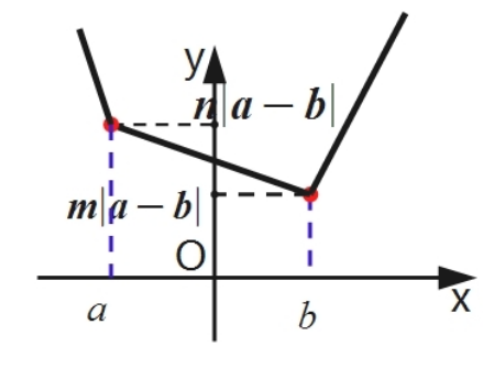
\includegraphics[width=\textwidth]{image20.png}
        \caption{\(m<n\)}
    \end{subfigure}
    \hfill
    \begin{subfigure}{0.45\textwidth}
        \centering
        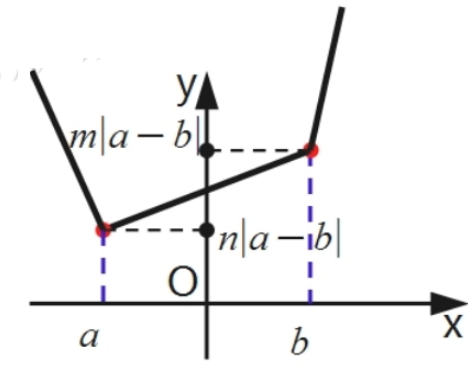
\includegraphics[width=\textwidth]{image21.png}
        \caption{\(m>n\)}
    \end{subfigure}
    \caption{歪底锅模型}\label{fgr:wddigomoxk}
\end{figure}

注意到,不论\(m,n\) 的大小关系如何,函数的最小值点总是为\(m,n\)中较大者对应绝对值内部关于 \(x\) 的表达式的零点。

\subsubsection{过山车模型}

客套话就不说了。\(f(x)=m|x-a|-n|x-b|\ (m,n>0,a\ne b)\)可分为下面两种情形:

(情形一)如图~\ref{fgr:goujiemoxk1},当\(a<b\)时,
\[f(x)=
    \begin{cases}
        (-m+n)x+am-bn, & x<a   \\
        na-nb,         & x=a   \\
        (m+n)x-am-bn,  & a<x<b \\
        -ma+mb,        & x=b   \\
        (m-n)x-am+bn,  & x>b
    \end{cases}
\]

\begin{figure}
    \centering
    \begin{subfigure}{0.45\textwidth}
        \centering
        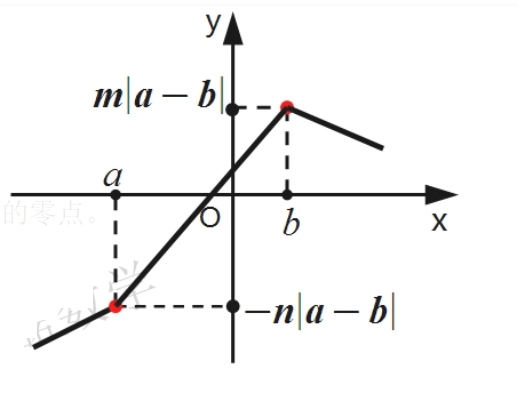
\includegraphics[width=\textwidth]{image22.png}
        \caption{\(m<n\)}
    \end{subfigure}
    \hfill
    \begin{subfigure}{0.45\textwidth}
        \centering
        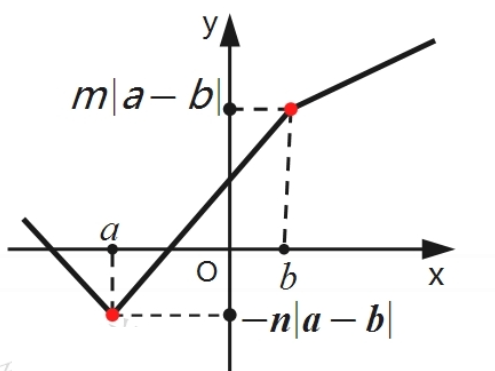
\includegraphics[width=\textwidth]{image23.png}
        \caption{\(m>n\)}
    \end{subfigure}
    \caption{过山车模型(\(a<b\))}\label{fgr:goujiemoxk1}
\end{figure}

(情形二)如图~\ref{fgr:goujiemoxk2},当 \(a>b\) 时,
\[f(x)=
    \begin{cases}
        (-m+n)x+am-bn, & x<b   \\
        ma-mb,         & x=b   \\
        (-m-n)x+am+bn, & b<x<a \\
        -na+nb,        & x=a   \\
        (m-n)x-am+bn,  & x>a
    \end{cases}
\]

\begin{figure}
    \centering
    \begin{subfigure}{0.45\textwidth}
        \centering
        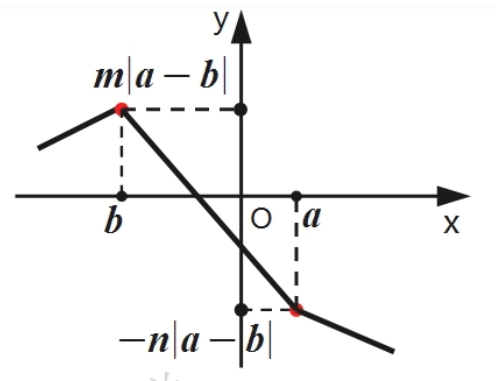
\includegraphics[width=\textwidth]{image24.png}
        \caption{\(m<n\)}
    \end{subfigure}
    \hfill
    \begin{subfigure}{0.45\textwidth}
        \centering
        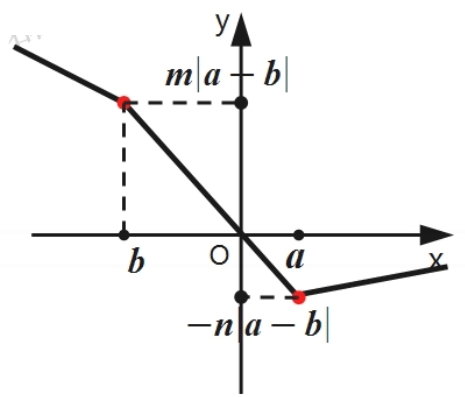
\includegraphics[width=\textwidth]{image25.png}
        \caption{\(m>n\)}
    \end{subfigure}
    \caption{过山车模型(\(a>b\))}\label{fgr:goujiemoxk2}
\end{figure}

注意到,不论 \(a,b\)大小如何,\marginpar{\footnotesize 猜你想找:二次函数二次项系数与开口方向。} %
\(m,n\) 中较大者对应项前符号为正则有最小值,为负则有最大值,最大(或小)值点总是为\(m,n\)中较大者对应绝对值内部关于 \(x\) 的表达式的零点。

\section{指数函数与对数函数}

本节研究内容限定在实数域内。

\subsection{指数}

\subsubsection{根式}

一般地,如果 \(x^n=a\),那么 \(x\) 叫作 \(a\) 的 \textbf{\(n\)次方根},其中 \(n>1,n \in \mathbb{N} ^*\)。

当 \(n\) 是奇数时,正数 \(n\) 次方根是一个正数,负数的 \(n\) 次方根是一个负数。这是 \(a\) 的 \(n\) 次方根用符号 \(\sqrt[n]{a}\) 表示。

当 \(n\) 是偶数时,正数 \(n\) 次方根有两个,二者互为相反数,正的用 \(\sqrt[n]{a}\) 表示,负的用 \(-\sqrt[n]{a}\)表示。二者可以合并写
作 \(\pm \sqrt[n]{a}\ (a>0)\)。负数没有偶次方根。

\(0\) 的任何次方根都为 \(0\),记作 \(\sqrt[n]{0}=0\)。

式子 \(\sqrt[n]{a}\)叫作\textbf{根式}\index{根式 radical},这里 \(n\) 叫作\textbf{根指数},\(a\)叫作\textbf{被开方数}。

根据 \(n\) 次方根的意义,可得
\begin{align*}
    (\sqrt[n]{a})^n & =a                     \\
    \sqrt[n]{a^n}   & =\begin{cases}
                           a,   & n \text{为奇数} \\
                           |a|, & n\text{为偶数}
                       \end{cases}
\end{align*}

\subsubsection{分数指数幂}

为了推广后能保持原有的运算性质,我们规定
\begin{gather*}
    a^{\frac{m}{n}}=\sqrt[n]{a^m}\ (a>0,\, m,n\in \mathbb{N} ^*,\, n>1)\\
    a^{-\frac{m}{n}}=\frac{1}{a^{\frac{m}{n}}}=\frac{1}{\sqrt[n]{a^m}}\ (a>0,\, m,n\in \mathbb{N} ^*,\, n>1)
\end{gather*}

规定:\(0\)的正分数指数幂等于 \(0\),\(0\)的负分数指数幂没有意义。

至此,因为所有有理数都可以表示为两个整数之比,所以我们已经把指数推广到了有理数域。

\subsubsection{无理数指数幂}

由于 \(\mathbb{Q} \) 在 \(\mathbb{R} \) 中稠密,换句话说,\(\forall x\in \mathbb{R} \),\(x\)都可以由 \(\mathbb{Q} \)中的数逼近,因此我们可以分别构造
单调递增和单调递减收敛于 \(x\) 的有理数序列\(\{r_n\},\{s_n\}\),再结合夹挤定理\marginpar{\footnotesize 夹挤定理,又称夹逼定理、夹极限定理、三明治定理、逼近定
    理、迫敛定理,指出若有两个函数在某点的极限相同,且有第三个函数的值在这两个函数之间,则第三个函数在该点的极限也相同。}与函数\(y=a^x\ (a>0)\)的连续性,可以确认
\(\{a^{r_n}\},\{a^{s_n}\}\)收敛于同一极限 \(a^x\),注意到结论与 \(x\) 是否为有理数无关,我们已经推广分数指数幂到无理数指数幂。

实数指数幂有如下运算性质:\(\forall r,s \in \mathbb{R} \),
\begin{align*}
    a^r a^s & =a^{r+s}\ (a>0)     \\
    (a^r)^s & = a^{rs}\ (a>0)     \\
    (ab)^r  & =a^r b^r\ (a>0,b>0)
\end{align*}

\subsection{指数函数}

\subsubsection{指数函数的定义}

形如 \(y=a^x\ (a>0\text{且}x\ne 1)\) 的函数叫作\textbf{指数函数}\index{指数函数 exponential function},其中 \(x\) 为自变量,定义域为 \(\mathbb{R} \)。

在实际问题中,经常会遇到指数增长和指数衰减,分别指的是增长率和衰减率为定值的变化模型,其中增长率或衰减率,是指一段时间过后,某一量的变化量与初始量之比。%
\footnote{增长率的另一个意思是瞬时增长速率,作为区分,此处沿用人教A版的解释。人教B版未出现此概念。}%
这类模型中,\(x\)次经过某一段时间后,终末量 \(y\) 与初始量 \(N\) 有如下关系:\(y=N(1+p)^x\ (x\in \mathbb{N} )\),其中\(p\)是增长率或衰减率(取相反数)。%
\footnote{事实上,这里应该为几何式增长,几何式增长处理的是离散时间(即增长率为定值),而指数增长处理的是连续时间(即瞬时增长速率与当前数量成正比)。教材未作区分。}

\subsubsection{指数函数的图象和性质}

在同一个坐标系下画出函数 \(y=a^x\) 与 \(y=\left( \dfrac{1}{a} \right)^x\ (a>1)\) 的图象,图~\ref{828db3ce-9b02-4441-a36c-c50cdfa31f41} 是 \(a=2\) 的情况。

因为 \(y={\left( \dfrac{1}{2} \right)}^x=2^{-x}\),点 \((x,y),(-x,y)\) 关于 \(y\) 轴对称,所以 \(y=2^x\) 图象上任意一点 \(P(x,y)\) 关于 \(y\) 轴的对称
点 \(P'(-x,y)\) 都在函数 \(y={\left( \dfrac{1}{2} \right)}^x\) 的图象上;反之亦然。由此可知,底数互为倒数的两个指数函数的图象关于 \(y\) 轴对称。
\label{329e9729-2614-4d87-809f-317659c55a0d}

事实上,指数函数的图象根据底数 \(a\) 的取值,可分为 \(0<a<1\) 和 \(a>1\) 两种类型,如表~\ref{tbl:viuuhjuutuxlxkvi} 所示。

\begin{table}
    \begin{tabular}{|c|c|c|} \hline
        项目   & \(0<a<1\)                                          & \(a>1\)                                            \\ \hline
        图象   & 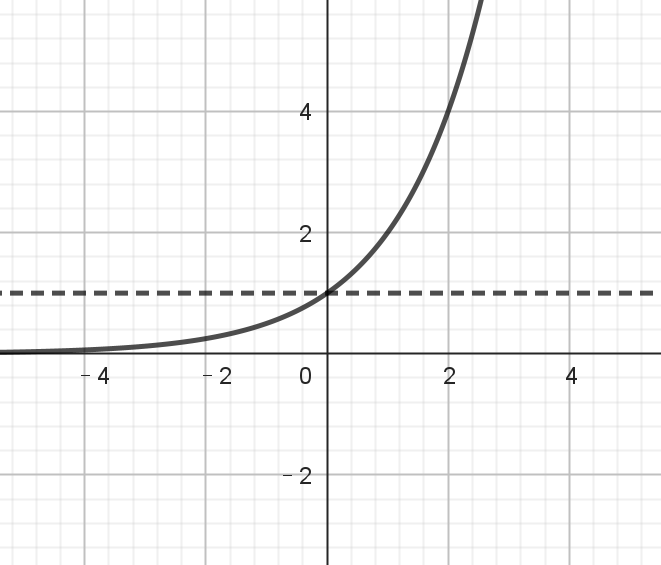
\includegraphics[width=0.4\textwidth]{image27.png} & 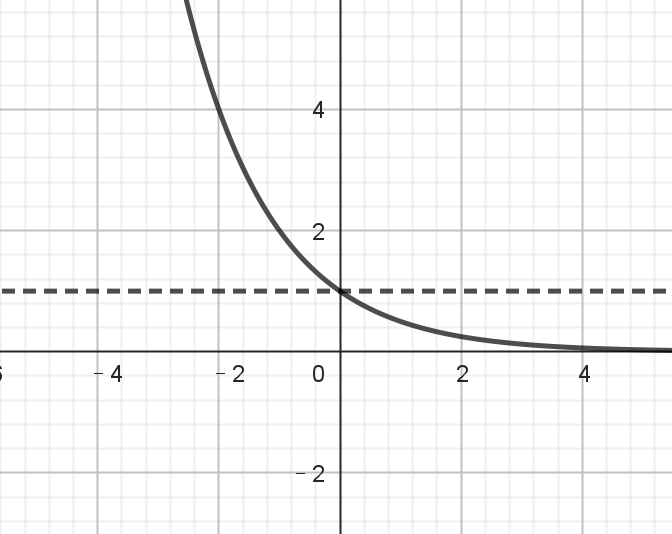
\includegraphics[width=0.4\textwidth]{image28.png} \\ \hline
        定义域 & \multicolumn{2}{c|}{\(\mathbb{R} \)}                                                                    \\ \hline
        值域   & \multicolumn{2}{c|}{\((0,+\infty )\)}                                                                   \\ \hline
        过定点 & \multicolumn{2}{c|}{\((0,1)\)}                                                                          \\ \hline
        单调性 & 减函数                                             & 增函数                                             \\ \hline
    \end{tabular}
    \caption{指数函数的图象与性质} \label{tbl:viuuhjuutuxlxkvi}
\end{table}

合理利用指数函数的单调性,通过自变量的大小关系可以判断相应函数值的大小关系。

\begin{figure}
    \centering
    \begin{minipage}{0.4\textwidth}
        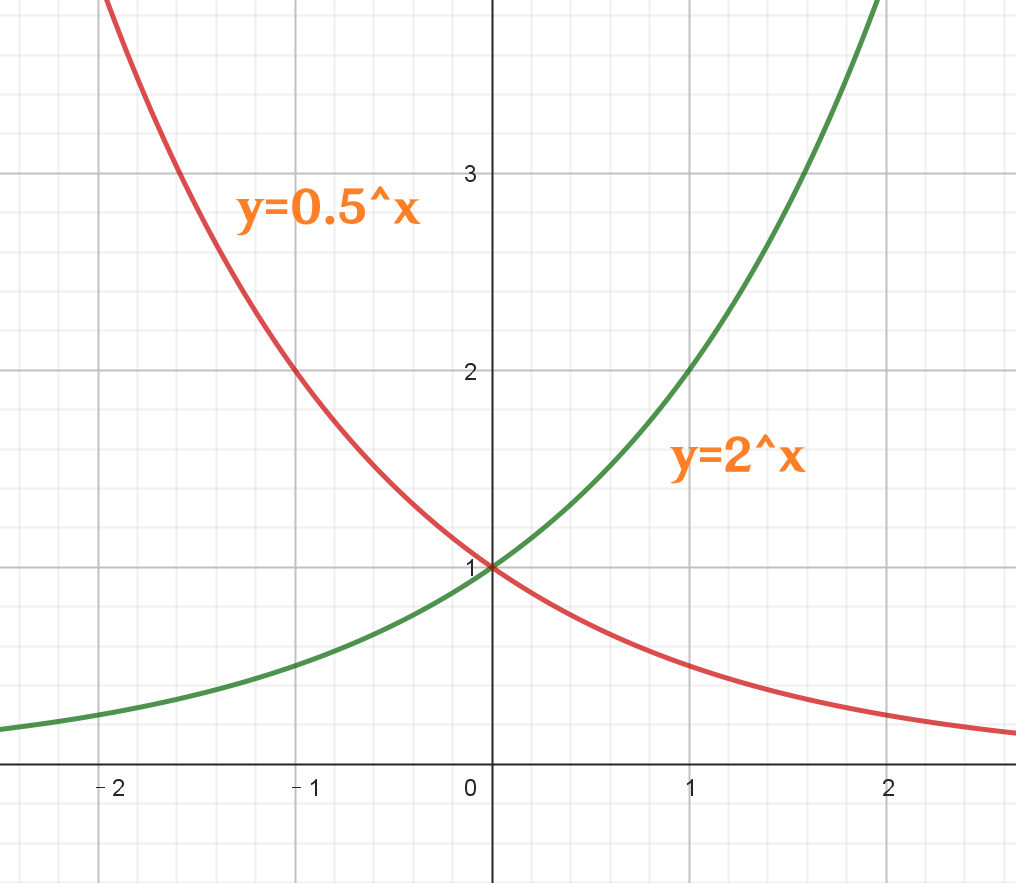
\includegraphics[width=\textwidth]{image26.png}
        \caption{指数函数的图象}\label{828db3ce-9b02-4441-a36c-c50cdfa31f41}
    \end{minipage}
    \hfill
    \begin{minipage}{0.5\textwidth}
        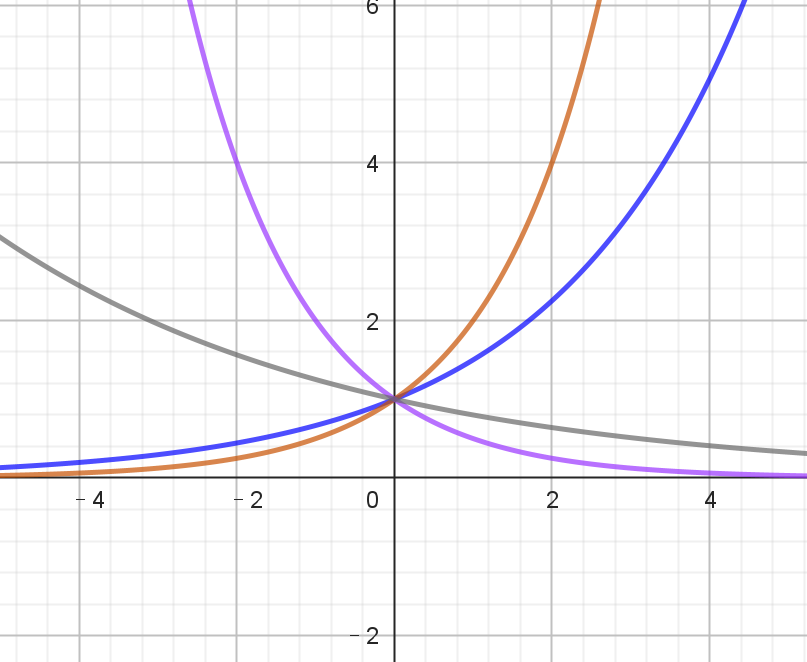
\includegraphics[width=\textwidth]{image29.png}
        \caption{不同底数指数函数的图象}\label{176e6d9b-3a3e-46eb-9777-99749aabcc01}
    \end{minipage}
\end{figure}

如果底数不同的指数函数图象出现在同一个坐标系下,可以利用 \(a^1=a\) 的性质,作出直线 \(x=1\) 来判断底数的大小关系,此时与函数图象交点 \((1,a)\) 的纵坐标
即为 \(a\) 的值,如图~\ref{176e6d9b-3a3e-46eb-9777-99749aabcc01} 所示。事实上,除 \(1\) 以外,任何正数都可作为竖直线的横坐标,因为 \(y=x^t\ (t>0)\) 是增函数。

\subsection{对数}

\subsubsection{对数的定义}

一般地,如果 \(a^x=N\,(a>0,a\ne 1)\),那么 \(x\) 叫作以 \(a\)为底\(N\) 的\textbf{对数}\index{对数 logarithm},记作 \(x=\log_a N\),其中 \(a\) 叫
作对数的\textbf{底数},\(N\)叫作真数。

通常,我们把以 \(10\) 为底的对数叫作\textbf{常用对数}\index{常用对数 common logarithm},并把 \(\log_{10} N\) 简记为\(\lg N\)。以 \(e\) 为底的对数
称为\textbf{自然对数}\index{自然对数 natural logarithm},并把 \(\log_e N\) 简记为 \(\ln N\)。

根据对数的定义,当 \(a>0,a\ne 1\) 时,\(a^x=N \Leftrightarrow x=\log_a N\)。

由指数与对数的这个关系,可以得到:负数和 \(0\) 没有对数;\(\log_a 1=0,\log_a a=1\)。

\subsubsection{对数的运算}

设 \(M=a^m,N=a^n\),因为 \(a^m a^n=a^{m+n}\),所以 \(MN=a^{m+n}\)。这样,就得到了对数运算的和公式。类似的,可以得到对数的差公式和次方公式。

如果 \(a>0,a\ne 1, M>0,N>0\),那么
\begin{align*}
    \log_a(MN)          & =\log_a M+\log_a N     \\
    \log_a \dfrac{M}{N} & = \log_a M - \log_a N  \\
    \log_{a^m} M^n      & = \dfrac{n}{m}\log_a M
\end{align*}

设 \(\log_a b=x\),则 \(a^x=b\),于是 \(\log_c a^x=\log_c b\),应用次方公式得 \(x\log_c a=\log_c b\),于是我们得到了\textbf{对数换底公式}:
\[
    \log_a b=\dfrac{\log_c b}{\log_c a}\ (a>0,a\ne 1,b>0,c>0,c\ne 1)
\]

\subsection{对数函数}

\subsubsection{对数函数的定义}

一般地,形如 \(y=\log_a x\ (a>0,a\ne 1)\) 的函数叫作\textbf{对数函数}\index{对数函数 logarithmic function},其中 \(x\) 是自变量,定义域是 \((0,+\infty )\)。

\subsubsection{对数函数的图象与性质}

与研究指数函数一样,我们先画出图象,再借助图象研究其性质。图~\ref{eec40c13-e9b5-44b4-8c1a-7912803aa638} 是底数为 \(2\) 的对数函数图象。

\begin{figure}
    \centering
    \begin{minipage}{0.4\textwidth}
        \centering
        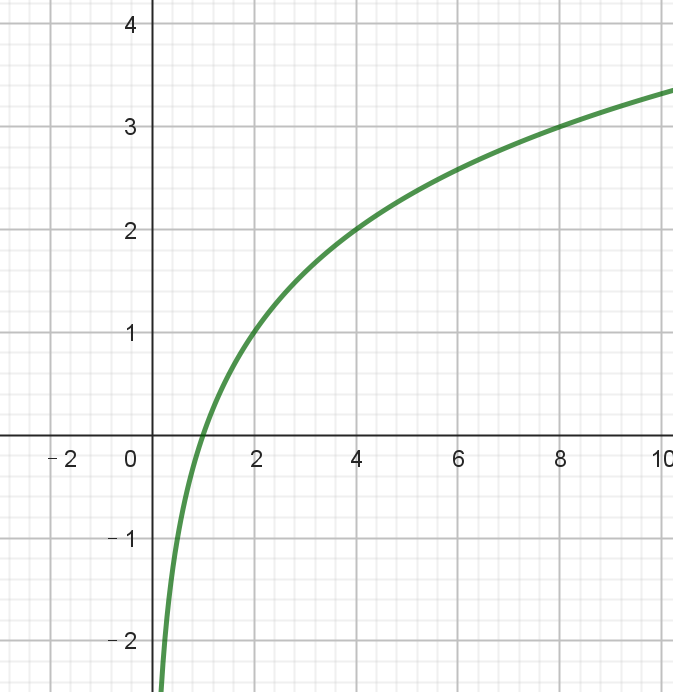
\includegraphics[width=\textwidth]{image30.png}
        \caption{\(y=\log_2 x\)}\label{eec40c13-e9b5-44b4-8c1a-7912803aa638}
    \end{minipage}
    \hfill
    \begin{minipage}{0.4\textwidth}
        \centering
        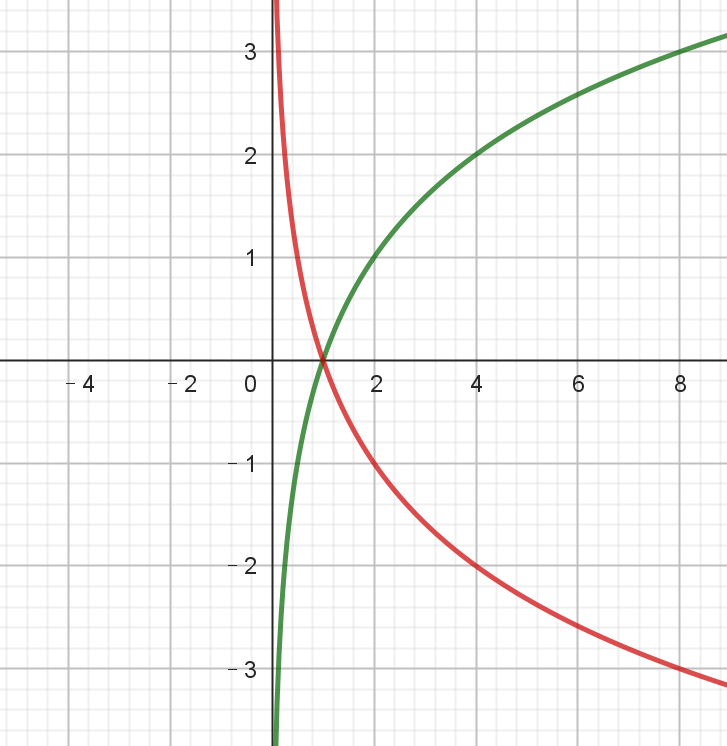
\includegraphics[width=\textwidth]{image31.png}\
        \caption{\(y=\log_{\frac{1}{2}} x\)}\label{173fd789-10db-41a1-9363-807ea6703850}
    \end{minipage}
\end{figure}

应用次方公式,可以得到 \(y=\log_{\frac{1}{2}} x=-\log_2 x\)。在同一坐标系中作出两个函数的图象,如图~\ref{173fd789-10db-41a1-9363-807ea6703850} 所示。
与~\ref{329e9729-2614-4d87-809f-317659c55a0d} 节同理,可以得到,底数互为倒数的两个对数函数的图象关于 \(x\) 轴对称。

类似于指数函数,对数函数的图象根据底数 \(a\) 的取值,也可分为 \(0<a<1\) 和 \(a>1\) 两种类型。对数函数的性质数表~\ref{tbl:dvuuhjuudetuxlyuxkvi} 所示。

\begin{table}
    \begin{tabular}{|c|c|c|} \hline
        项目   & \(0<a<1\)                                          & \(a>1\)                                            \\ \hline
        图象   & 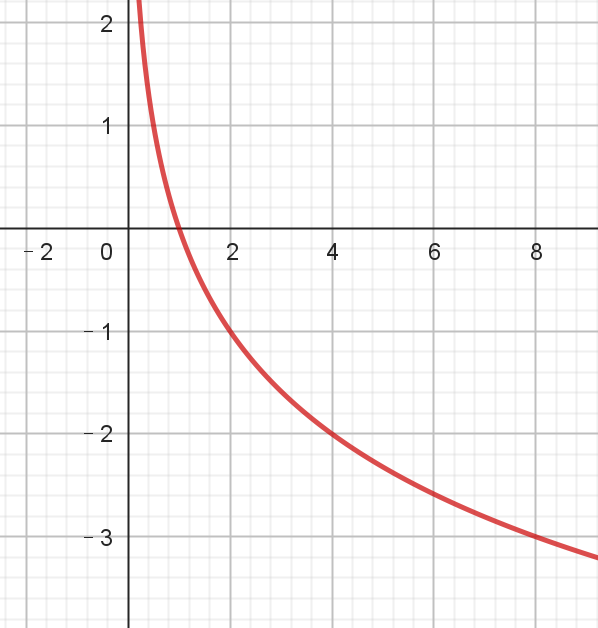
\includegraphics[width=0.4\textwidth]{image32.png} & 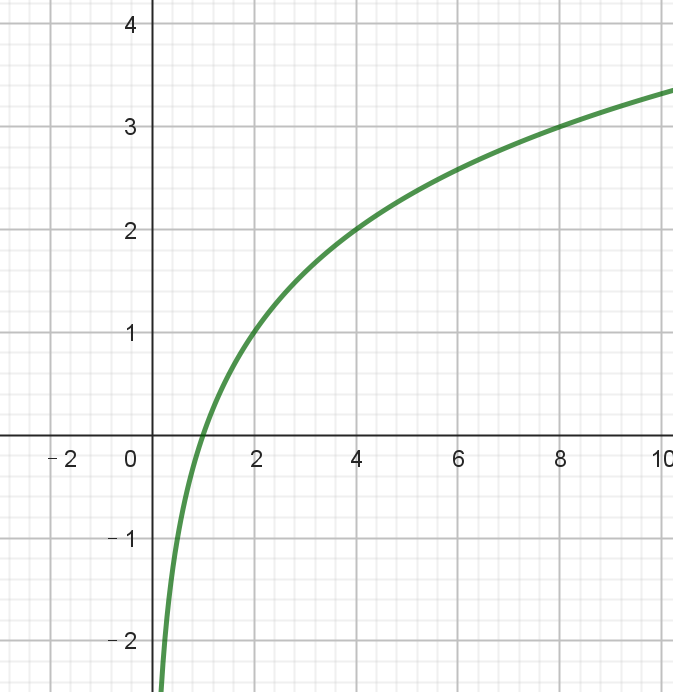
\includegraphics[width=0.4\textwidth]{image30.png} \\ \hline
        定义域 & \multicolumn{2}{c|}{\((0,+\infty )\)}                                                                   \\ \hline
        值域   & \multicolumn{2}{c|}{\(\mathbb{R} \)}                                                                    \\ \hline
        过定点 & \multicolumn{2}{c|}{\((1,0)\)}                                                                          \\ \hline
        单调性 & 减函数                                             & 增函数                                             \\ \hline
    \end{tabular}
    \caption{对数函数的图象与性质} \label{tbl:dvuuhjuudetuxlyuxkvi}
\end{table}

在同一坐标系内,如果有多个对数函数的图象,可作出直线 \(y=1\),底数大的对数函数与直线的交点横坐标大,反之亦然。

\section{反函数与不同函数增长差异}

\subsection{反函数的定义}

反函数,也称作逆函数,是对某个函数做逆运算的函数。

设函数 \(f:X\to Y\)。如果存在一个函数 \(g:Y\to X\),并 \(\forall x \in X,g(f(x))=x\) 且 \(\forall y\in Y,f(g(y))=y\),
则称 \(g\) 为 \(f\) 的\textbf{反函数}\index{反函数 inverse function},记之为 \(f^{-1}\)。若一函数有反函数,称此函数可逆。

这就是说,沿用函数就像机器的比喻,一个函数 \(f\) 存在反函数 \(g\),需要 \(g\) 就像“撤销工具”,能把 \(f\) 执行的操作“撤销”掉、给出原有的唯一确定的 \(x\),并且能且仅能撤
销 \(f\) 可能执行的所有操作。这告诉我们,\(f\)要想拥有反函数\(g\),必须要保证不存在两个不同的输入给出相同的输出,否则把这个输出给反函数 \(g\),又怎么知道
哪一个才是真正的输入呢?另一方面,需要 \(f\) 的值域与到达域 \(Y\)相等,即 \(\forall y \in Y,\exists x\in X, f(x)=y\)。这是因为,由定义,\(g\)应当能撤销 \(Y\)
中所有的元素的操作,但是要是 \(f\) 执行操作根本给不出某个元素 \(y\in Y\),那么把这个“输出” \(y\) 放到“撤销工具”里,又会得到什么样的结果呢?进一步,如果再把这个撤销
结果输入给 \(f\),又该如何是好呢?

这告诉我们,一个函数可逆的充分必要条件是该函数为双射,即同时为

\begin{itemize}
    \item 单射:\(\forall x_1,x_2\in X,\ f(x_1)=f(x_2)\Rightarrow x_1=x_2\)。
    \item 满射:\(\forall y\in Y,\exists x\in X, \ f(x)=y\)。
\end{itemize}

验证一个函数是否为双射(也就可逆)的方法是水平线检验法,也就是函数图象须和纵坐标在到达域内的任何一条水平线有且仅有一个交点。

\subsection{反函数的性质}

反函数具有如下性质:

\begin{enumerate}
    \item 原函数的定义域、值域分别是反函数的值域、定义域;
    \item 原函数与其反函数的函数图象关于直线 \(y=x\) 对称;
    \item 单调函数一定存在反函数,且反函数与原函数的单调性一致;
    \item 拥有反函数的函数不一定是单调函数,例如 \(y=x^{-3}\)。
\end{enumerate}

一部分函数尽管本身不可逆,但它到其定义域的某个子集上的限制\marginpar{\footnotesize 映射 \(f\) 的限制是一个新的映射,记
    作 \(f|_A\) 或 \(f \upharpoonright _A\),它是通过为 \(f\) 选择一个更小的定义域 \(A\) 得到的。反过来,也称 \(f\) 是映射 \(f|_A\)的扩张。}%
是可逆的。也就是说,对这类函数,如果我们限制其定义域到某一范围内,则限制后的函数可逆。

\subsection{不同函数增长的差异}

如图~\ref{fgr:sjvshjuuzgvhsudu},在同一坐标系内画出指数函数、幂函数与对数函数的图象,并改变坐标尺到一个较大的范围。可以
看出,当 \(x\) 足够大时,有指数函数\(>\)幂函数 \(>\) 对数函数。那么是不是对任意的指数函数、幂函数和对数函数都有这样的结论呢?

\begin{figure}
    \centering
    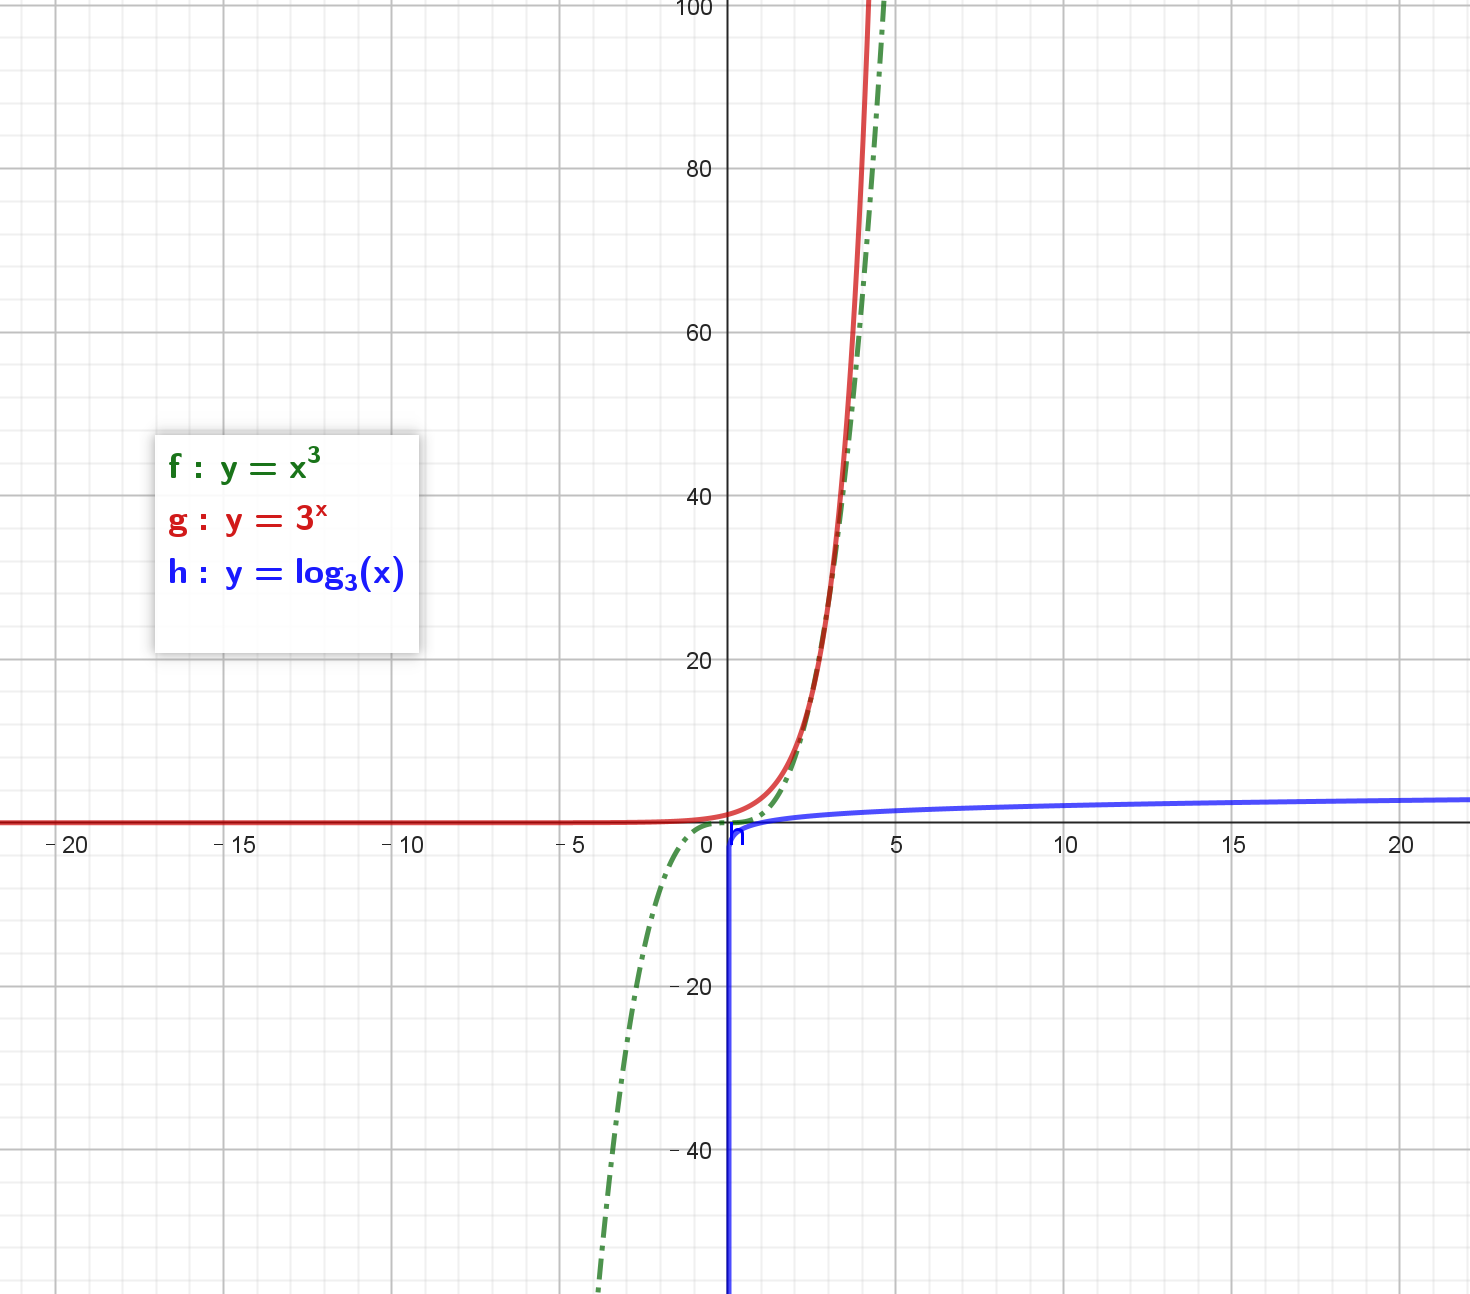
\includegraphics[width=0.8\textwidth]{image33.png}
    \caption{三种函数增长速度}\label{fgr:sjvshjuuzgvhsudu}
\end{figure}

\section{函数、方程、不等式之间的关系}

\section{函数的应用}

\subsection{对数函数:世界是对数的}

\subsection{指数函数:曾“几何”时}

\subsection{幂函数:规模效应}

\subsection{三角函数:波动的谐律}

\subsection{二次函数:宇宙之“2”}

\subsection{再看函数:混沌中的确定}

\chapter{导数}

\chapter{平面向量、解三角形}

\chapter{立体几何}

\chapter{解析几何}

\chapter{排列组合}

\chapter{数列}

\chapter{统计与概率}

\appendix

\chapter{B版中的阅读材料}

本附录收录了人教版B版高中教材中的部分阅读材料,作为补充阅读之用,顺序大致与本书内容对应。\marginpar{\footnotesize 我们A版学生也是太悲催了}

\section{利用复数产生分形图(复变函数)}

以前我们学过的函数,定义域都是实数集的子集.但函数概念还可以推广:定义域是复数集的子集的函数称为复变函数。类似地,我们还可以得到多项式复变函数的概念。例如,%
\(f(z)=z^2\) 就是一个多项式复变函数,此时 \(f(\ii)=\ii^2=-1,f(1+\ii)=(1+\ii)^2=2\ii\)。

给定多项式复变函数 \(f(z)\) 之后,对任意一个复数 \(z_0\),通过计算公式 \(z_{n+1}=f(z_n),n\in \mathbb{N}\) 可以得到一列值 \(z_0,z_1,z_2,\dots,z_n,\dots\)。

如果存在一个正数 \(M\),使得 \(|z_n|<M\) 对任意 \(n\in \mathbb{N}\) 都成立,则称 \(z_0\) 为 \(f(z)\) 的收敛点;否则,称 \(z_0\) 为 \(f(z)\) 的发散点。%
\(f(z)\) 的所有收敛点组成的集合称为 \(f(z)\) 的充满茹利亚集。

例如,当\(f(z)=z^2\)时,如果\(z_0=\ii\),则得到的一列值是 \(\ii,-1,1,1,\dots,1,\dots\);如果 \(z_0=1+\ii\),则算出的一列值是\(1+\ii,2\ii,-4,\dots,2^{2^{n-1}},\dots\)。

显然,对于\(f(z)=z^2\) 来说,\(\ii\) 为收敛点,\(1+\ii\)为发散点。事实上,利用\(|z^2|=|z|^2\)可以证明,\(f(z)=z^2\)的充满茹利亚集是一个单位圆盘(即由
满足\(|z|\le 1\)的所有\(z\)组成的集合)。

让人惊讶的是,当\(f(z)=z^2+c\)时,对于某些复数\(c\)来说,\(f(z)\)的充满茹利亚集是非常复杂的。如果利用计算机对不同形态的收敛点和发散点进行不同的着色,就
可以得到与本章导语所示类似的分形图.而且,如果按照一定的规则对\(c\)进行分类,并进行着色,可以得到如图~\ref{fgr:mhdebuloffxktu} 所示的芒德布罗分形图。

\begin{figure}
    \centering
    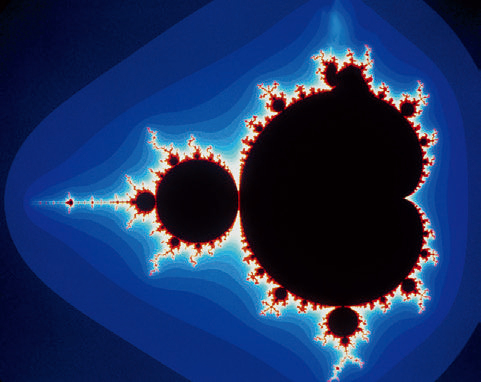
\includegraphics[width=0.4\textwidth]{image6.png}
    \caption{芒德布罗分形图}\label{fgr:mhdebuloffxktu}
\end{figure}

\section{四元数简介}

数学中的数,除了实数、复数之外,还有四元数。一般地,形如 \( a + b\mathrm{i} + c\mathrm{j} + d\mathrm{k} \) 的数为
四元数,其中 \( a, b, c, d \) 都是实数,$\mathrm{i}$, $\mathrm{j}$, $\mathrm{k}$ 都是虚数单位,这些虚数单位满足
\[ \mathrm{i}^2 = \mathrm{j}^2 = \mathrm{k}^2 = -1 \]

给定两个四元数,可以进行同复数类似的加法和减法运算,例如
\[ (2 + 3\mathrm{i} + 4\mathrm{j} + 5\mathrm{k}) + (6 + 7\mathrm{i} + 8\mathrm{j} + 9\mathrm{k}) = 8 + 10\mathrm{i} + 12\mathrm{j} + 14\mathrm{k}\]

不过,对于两个四元数相乘来说,情况就比复数相乘复杂得多。因为此时,除了会出现 \( \mathrm{i}^2, \mathrm{j}^2,
\mathrm{k}^2 \) 之外,还会出现 \( \mathrm{i}\mathrm{j}, \mathrm{i}\mathrm{k}, \mathrm{j}\mathrm{k},
\mathrm{j}\mathrm{i}, \mathrm{k}\mathrm{i}, \mathrm{i}\mathrm{j} \) 等。一般地,两个四元数相乘时,规定
\[
    \mathrm{i}\mathrm{j} = -\mathrm{j}\mathrm{i} = \mathrm{k},
    \quad
    \mathrm{j}\mathrm{k} = -\mathrm{k}\mathrm{j} = \mathrm{i},
    \quad
    \mathrm{k}\mathrm{i} = -\mathrm{i}\mathrm{k} = \mathrm{j}
\]

例如,
\begin{align*}
      & (2 + 3\mathrm{i} + 4\mathrm{j} + 5\mathrm{k})(6 + 7\mathrm{i} + 8\mathrm{j} + 9\mathrm{k}) \\
    = & (12 - 21 - 32 - 45) +(14 + 18 + 36 - 40)\mathrm{i}                                         \\
      & +(16 + 24 + 35 - 27)\mathrm{j} +(18 + 30 + 24 - 28)\mathrm{k}                              \\
    = & -86 + 28\mathrm{i} + 48\mathrm{j} + 44\mathrm{k}
\end{align*}

由此也可以看出,四元数的乘法是不满足交换律的。

不过,有意思的是,与复数的乘法能够表示平面直角坐标系中的旋转类似,四元数的乘法能够表示空间中的旋转。因此,四元数在
描述三维旋转、姿态方面有一些独特的优点,人们经常使用四元数去描述飞行器、机器人等的姿态。感兴趣的同学请自行查阅有关资料。

顺带提及的是,有同学可能会想:既然能有四元数,那有没有三元数呢?能不能规定形如 \(a + b\mathrm{i} + c\mathrm{j}\) 的
数为三元数呢?其中 \(a, b, c\) 都是实数,$\mathrm{i}$, $\mathrm{j}$ 都是虚数单位。对这个问题感兴趣的同学,可以考虑
一下此时 $\mathrm{i}$ 与 $\mathrm{j}$ 的积$\mathrm{i}\mathrm{j}$的结果是什么,由此是否出现矛盾,等等。

\section{素数个数与对数}

我们已经知道,像2、3、5、7这样只能被1和它自己整除的正整数称为素数(也称为质数)。例如,100以内的所有素数为
2、3、5、7、11、13、17、19、23、29、31、37、41、43、47、53、59、61、67、71、73、79、83、89、97。

探索素数出现的规律,是一些数学家非常关心的问题。特别地,设 \( x \) 是正整数,用 \(\pi(x)\) 表示不超过 \( x \) 的素数个数,寻找 \(\pi(x)\) 的近似表达式,历史上曾引起了很多数学家的注意。当然,我们可以取 \( x \) 为一些常数,然后求出 \(\pi(x)\) 的值来进行观察和归纳。

可能会让你感到惊讶的是,\(\pi(x)\) 的近似表达式与自然对数有关。事实上,数学家们已经证明,当 \( x \) 充分大时,
\[\pi(x) \approx \frac{x}{\ln x}\]

这一结果可以从下表中直观感受到。

\begin{table}[h]
    \centering
    \begin{tabular}{cccc}
        \toprule
        \( x \)   & \(\pi(x)\) & \(\frac{x}{\ln x}\) & 相对误差 \\
        \midrule
        1 000     & 168        & 145                 & 13.69\%  \\
        5 000     & 669        & 587                 & 12.26\%  \\
        10 000    & 1 229      & 1 086               & 11.64\%  \\
        50 000    & 5 133      & 4 621               & 9.97\%   \\
        100 000   & 9 592      & 8 686               & 9.45\%   \\
        500 000   & 41 538     & 38 103              & 8.27\%   \\
        1 000 000 & 78 498     & 72 382              & 7.79\%   \\
        5 000 000 & 348 513    & 324 150             & 6.99\%   \\
        \bottomrule
    \end{tabular}
\end{table}

注:如果 \( A \) 的近似值为 \( a \),那么相对误差指的是
\[\frac{|A-a|}{A} \times 100\%\]

\listoftheorems[ignoreall,show={thmlevel1},title=定理索引]\addcontentsline{toc}{chapter}{定理索引}

\printindex

\end{document}